\section{Internet Protocol (IP) version 4}

\subsection{Introduzione}
\begin{figure}[h!]
    \begin{minipage}{0.45\textwidth}
        \centering
        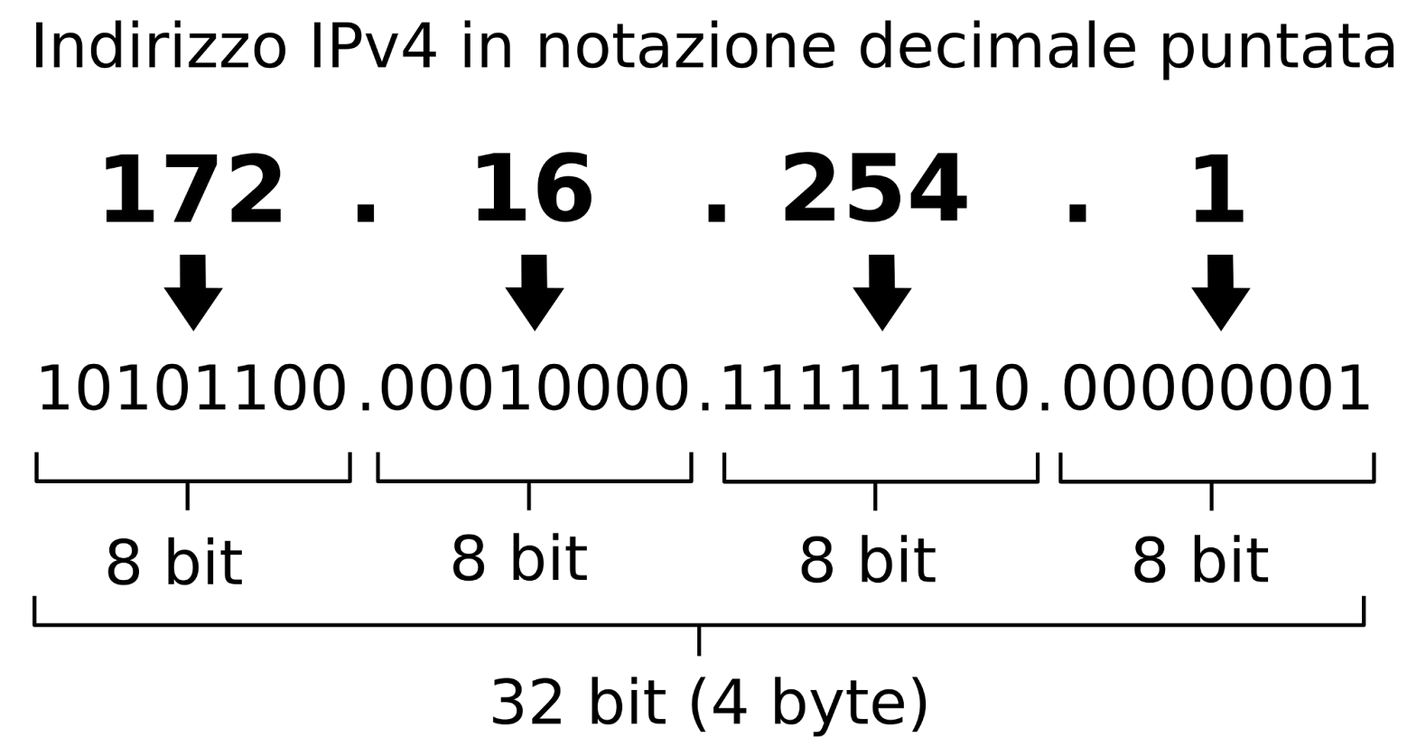
\includegraphics[width=0.95\textwidth]{images/indirizzoip.png}
        \caption{Struttura di un indirizzo IP}
        \label{fig:indirizzoip}
    \end{minipage}\hfill
    \begin{minipage}{0.52\textwidth}
        Al livello 3 ci preoccupiamo di trovare la strada migliore per raggiungere il destinatario.

        IPv4 è il protocollo di rete più diffuso al mondo, IP instrada i pacchetti immessi nella rete, ogni nodo in rete ha indirizzo ip.

        Ogni pdu(pacchetto) contiene gli indirizzi IP del host mittente e destinatario.
        
        IP è connectionless, ad inoltrare i pacchetti(datagram) sono i router, lo fanno attraverso algoritmi di routing(leggendo l’header del pacchetto). 

        Ip è inoltre “best-effort”, ossia fa del suo meglio, non garantisce affidabilità massima o ottimale.

        Gli indirizzi ip sono da 32 bit(4 numeri decimali compresi tra 0 e 255):
    \end{minipage}
\end{figure}

Gli host che appartengono alla stessa rete hanno in comune il livello fisico,
un dominio di broadcast è un insieme di computer di una stessa rete(stesso indirizzo ip di rete), esempio rete di casa(collegandoci al router di casa è possibile inviare un messaggio broadcast che arriverà a tutti i dispositivi che fanno parte della rete IP).
Le porte del router vengono chiamate interfacce, ogni interfaccia corrisponde ad un host;
ogni rete ha un indirizzo IP di rete.

\begin{figure}[h!]
    \centering
    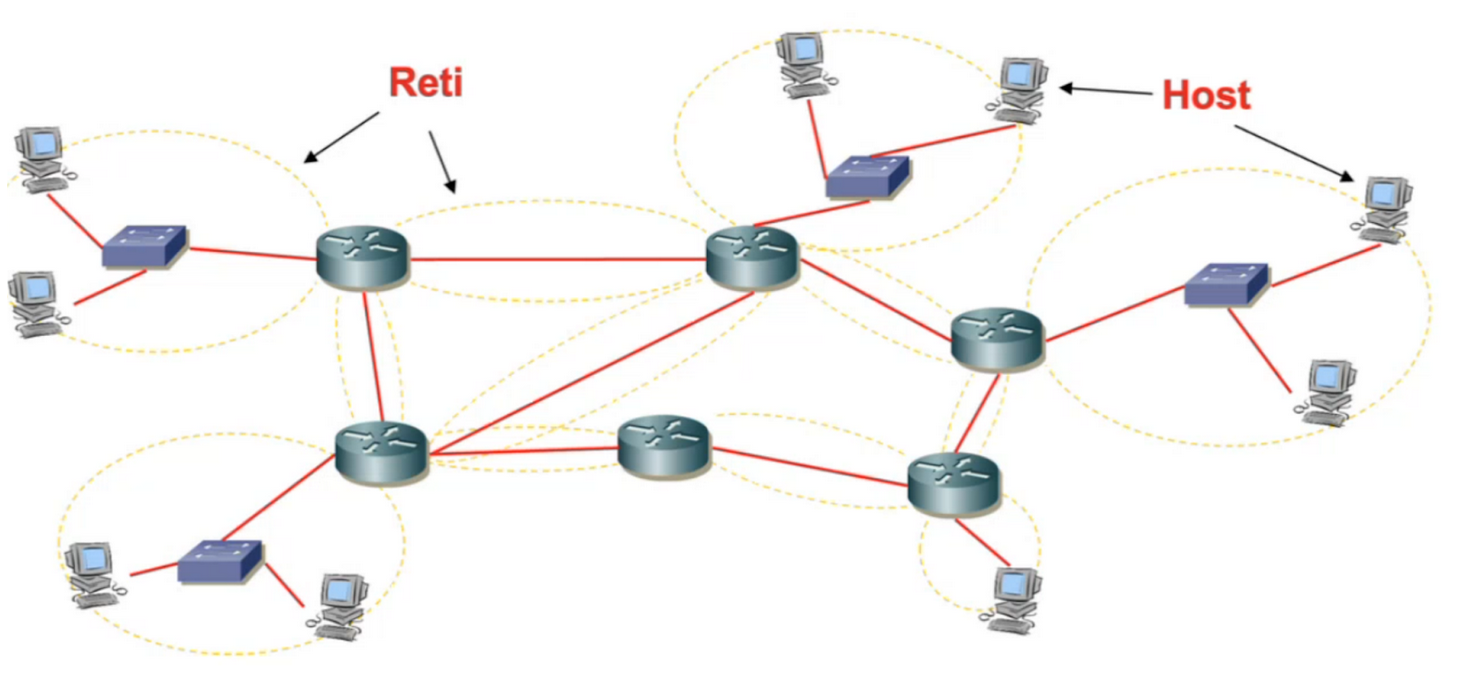
\includegraphics[width=0.59\textwidth]{images/reteipbase.png}
    \caption{Esempio di rete IP di base}
    \label{fig:reteipbase}
\end{figure}
\subsection{Datagramma IP}
I datagrams IP sono i pacchetti di dati che vengono inviati attraverso la rete utilizzando il protocollo IP. Ogni datagramma contiene un header e un payload. 
\begin{figure}[h!]
    \centering
    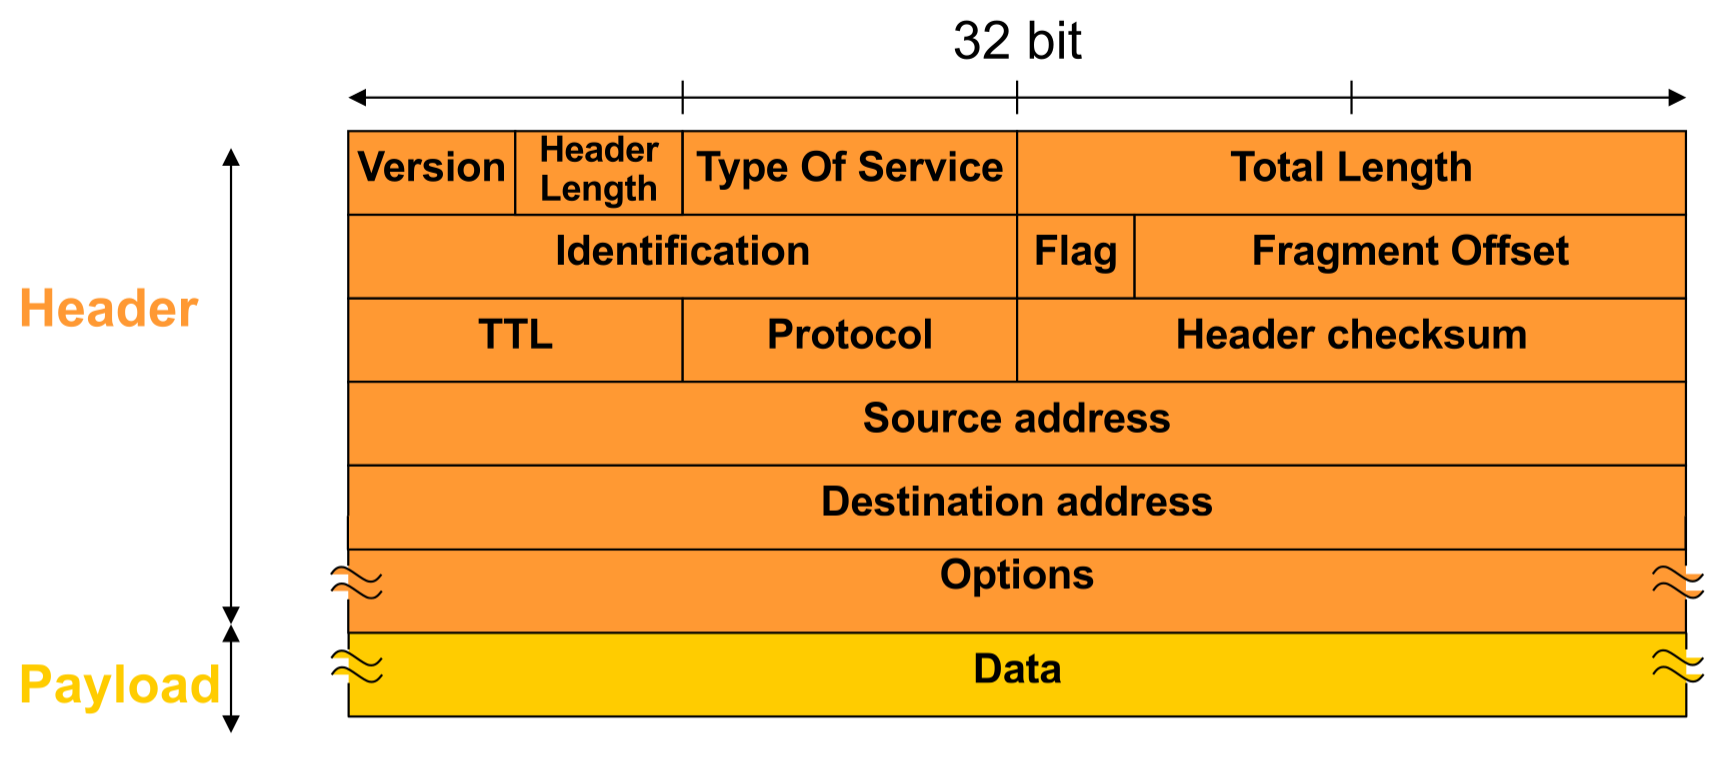
\includegraphics[width=0.9\textwidth]{images/datagrammaIP.png}
    \caption{Struttura di un datagramma IP}
    \label{fig:datagrammaIP}
\end{figure}

\begin{itemize}
    \item version: mi dice la versione del protocollo(IPv4 o IPv6) (è di 4 bit, mezzo byte)
    \item header legth: lunghezza del header (4 bit, mezzo byte), se voglio dire che l'header è lungo 5 posso scivere in questo campo 0101, che è 1 + 0 + 4 + 0
    \item type of service(TOS): (1 byte, 8 bit) distingue i tipi diversi di pacchetti, questo è utile nel momento in cui un router deve dare o no la precedenza a certi pacchetti, in base al tipo di servizio. esempio: precedenza al servizio x piuttosto che a y
    il TOS viene utilizzato per definire il liello di quality of service con cui trattare il pacchetto(primi 6 bit)(gli ultimi 2 servono ad evitare la congestione)
    
    \begin{figure}[h!]
        \centering
        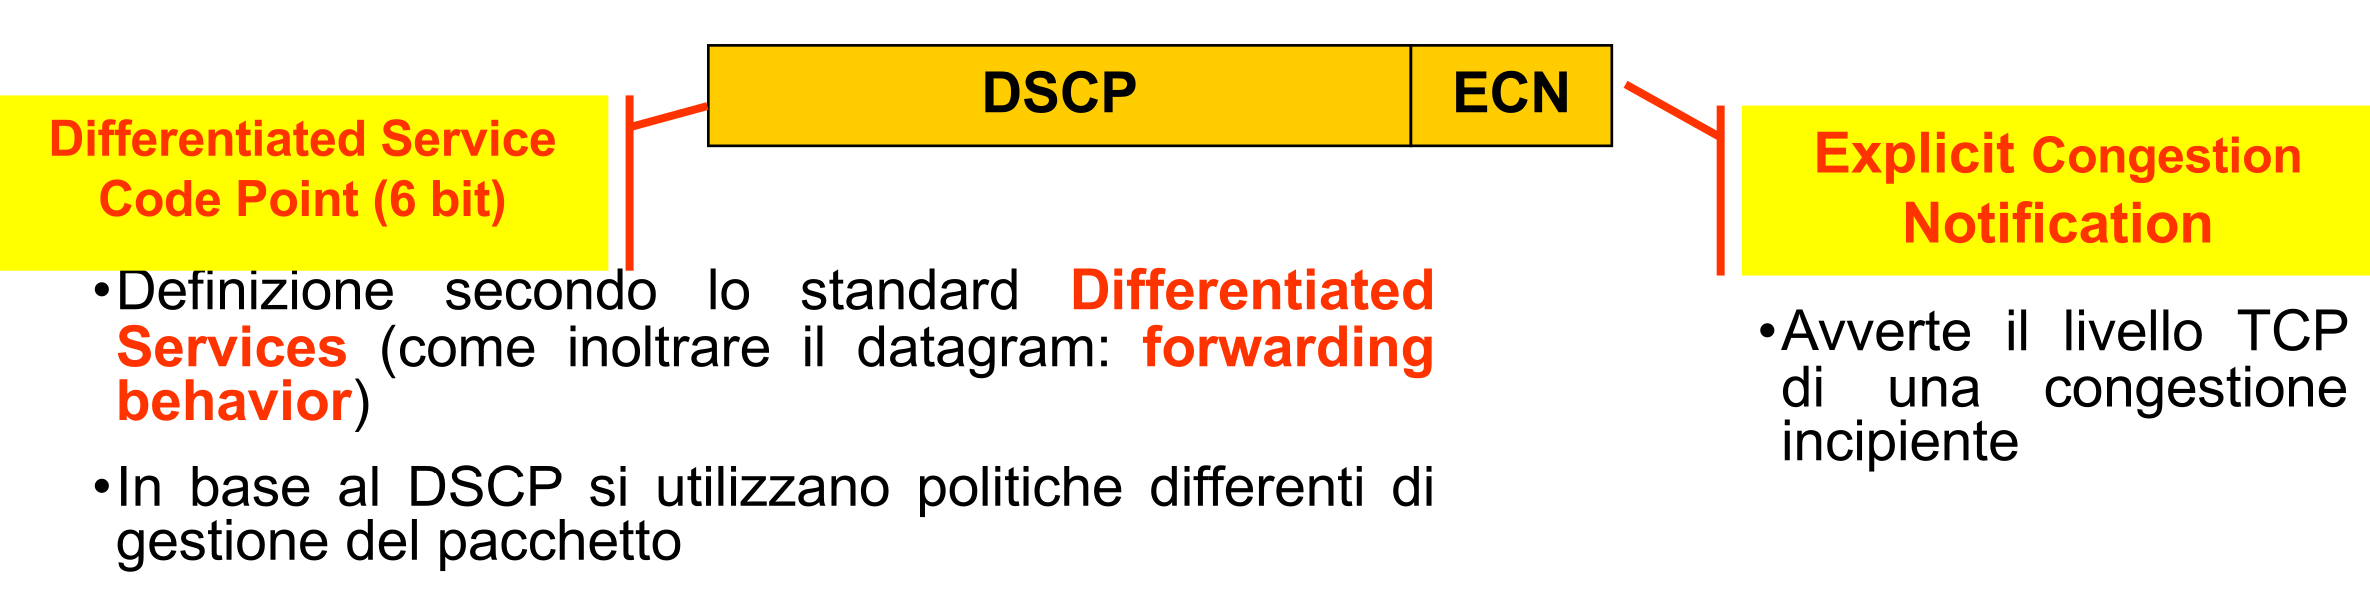
\includegraphics[width=1\textwidth]{images/tos.png}
        \caption{Campo Type of Service (ToS) nell'header IP}
        \label{fig:tos}
    \end{figure}

    \item total length:(16 bit) lunghezza del datagramma in byte(max 65535 byte)
    \item identification(16 bit) identifica in modo univoco un datagramma generato dal mittente, quindi anche se il pacchetto viene frammentato, i suoi “frammenti”, ossia altri pacchetti che contengono parte del payload iniziale, avranno lo stesso id. serve quindi a gestire la frammentazione dei pacchetti ip
    \item options: opzioni per il routing del pacchetto, è un campo poco usato per via del carico di elaborazione molto variabile
    \item data: è l'informazione da inviare
\end{itemize}
\newpage
\begin{itemize}
    \item flag(3 bit)
\end{itemize}
        \begin{figure}[h!]
            \begin{minipage}{0.55\textwidth}
                \raggedright
                 il primo bit non usato, il secondo bit è il flag DF (don't fragment: specifica che il router può frammentare il pacchetto o no), il terzo bit è il flag MF (more fragment: indica se il seguente datagramma è l'ultimo dei frammenti). Per utilizzare questi flag metto il valore del bit corrispondente al flag ad 1. Esempio: 010, 0 iniziale è indifferente, 1 indica il flag DF attivo, mentre lo 0 alla fine mi dice che non è MF, quindi che questo datagram è l'ultimo frammento.
            \end{minipage}\hfill
            \begin{minipage}{0.4\textwidth}
                \centering
                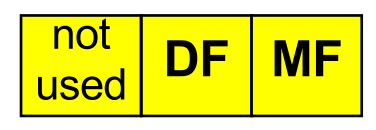
\includegraphics[width=\textwidth]{images/flagsIP.png}
                \caption{Campo Flags nell'header IP}
                \label{fig:flagsIP}
            \end{minipage}
        \end{figure}
\begin{itemize}
    \item fragment offset(13 bit) mi dice la posizione del frammento all'interno del pacchetto originario, lo spiazzamento. è espresso in multipli di 8 byte. 
\end{itemize}

    \begin{figure}[h!]
        \begin{minipage}{0.55\textwidth}
            \textbf{Frammentazione}: quando un datagramma IP deve attraversare una rete con una MTU (Maximum Transmission Unit) inferiore alla sua dimensione, viene suddiviso in frammenti più piccoli. Ogni frammento contiene parte dei dati originali e un header IP con informazioni per il riassemblaggio.

            Nella figura il pacchetto è grande 4000 byte(total length), in questo caso viene frammentato in 3 poichè la sua MTU vale 1500 byte , i frammenti condividono lo stesso id del pacchetto non frammentato.

            I frammenti devono avere un offset multiplo di 8.

            Solamente il primo frammento ha offset pari a 0, rappresenta la testa.
            Solamente l'ultimo frammento ha MF pari a 0 poichè sta ad indicare che quello è l'ultimo pezzo del pacchetto, la coda. CHIARIRE
        \end{minipage}\hfill
        \begin{minipage}{0.4\textwidth}
            \centering
            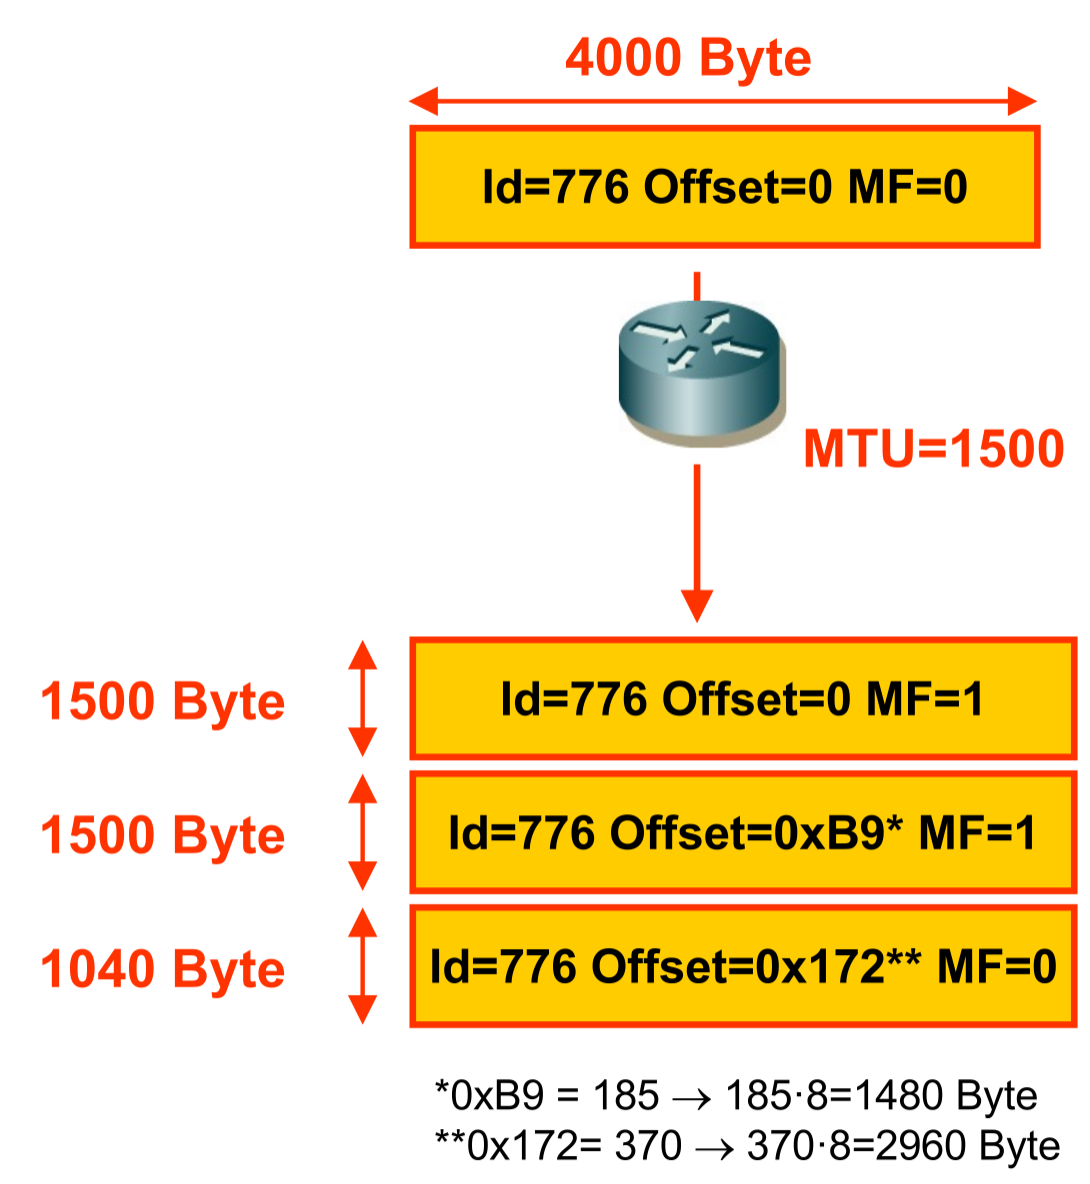
\includegraphics[width=\textwidth]{images/frammentazione.png}
            \caption{Esempio di frammentazione di un datagramma IP}
            \label{fig:frammentazioneIP}
        \end{minipage}
    \end{figure}

\begin{itemize}
    \item time to live(8 bit) evita il problema dei pacchetti che entrano in loop poichè non trovano il destinatario. è il tempo di vita del pacchetto, ogni router che riceve il pacchetto(ad ogni hop) decrementa il valore time to live, facendo così arriverà un punto in cui il time to live del pacchetto è stato decrementato fino a zero. quando arriva a 0 il datagram viene scartato. è un valore stabilito dal mittente(esempio 128)
    \item protocol(8 bit): contiene un numero che specifica il protocollo usato dalla PDU incapsulata dal datagram. esempio TCP = 6 . UDP = 17 $\rightarrow$ livello 4
    \item header checksum(16 bit): controlla i byte del header, è un controllo veloce su header. se c'è un errore sull'header allora il pacchetto viene scartato, come funziona? : somma 16 bit a 16 bit gli altri byte dell’header,fa la somma dell'eventuale resto e fa il complemento ad 1 del risultato.

Se non ci sono errori, la somma a 16 bit di tutti questi valori deve dare come risultato 0xFFFF (cioè tutti i bit a 1).

\item source/destination address: (32 bit) è l'indirizzo ip del mittente/destinatario

\end{itemize}

\subsubsection{Struttura indirizzo IP}
\begin{figure}[h!]
    \centering
    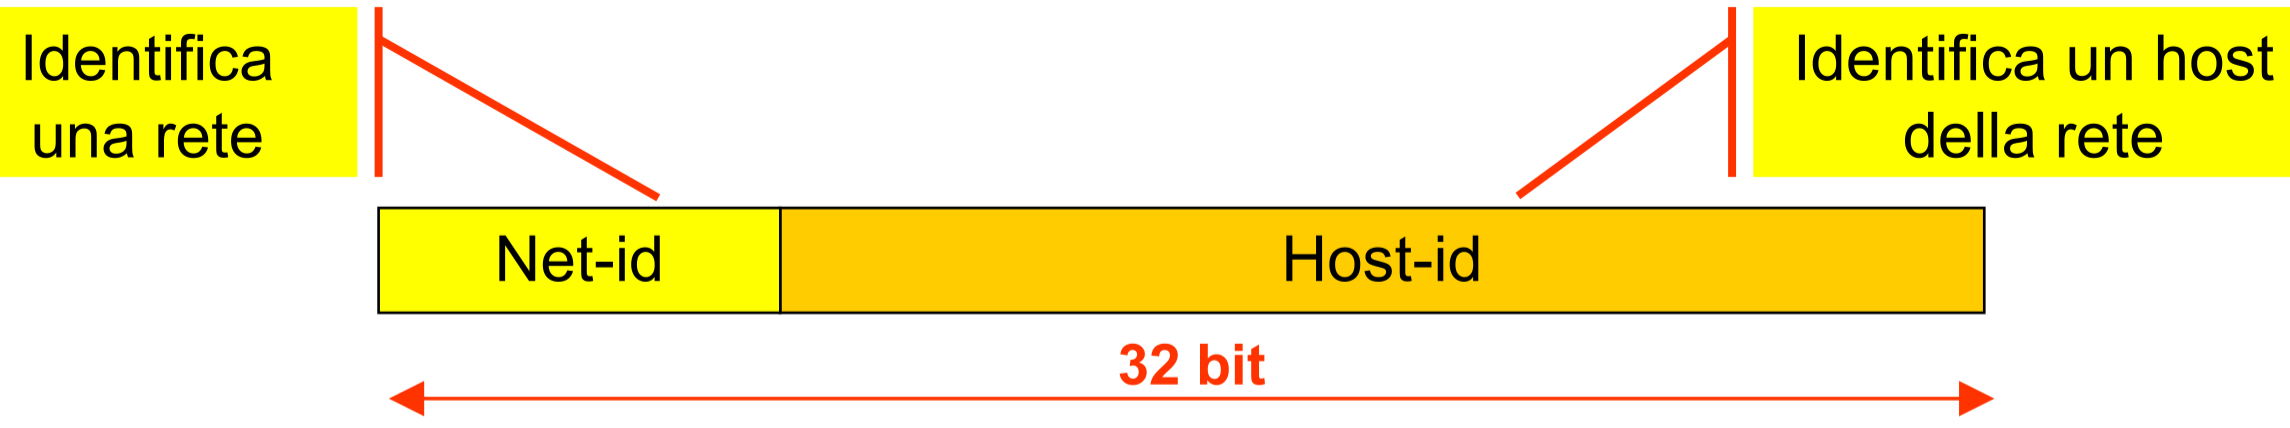
\includegraphics[width=0.8\textwidth]{images/strutturaIP.png}
    \caption{Struttura di un indirizzo IP: suddivisione in parte di rete e parte host}
    \label{fig:strutturaIP}
\end{figure}

Attualmente si utilizza l'indirizzamento classless CIDR (Classless Inter-Domain Routing), che permette di specificare la lunghezza della maschera di rete in bit.

L'assegnazione degli indirizzi è compito dell'Internet Assigned Number
Authority (IANA) gestita dall'ICANN (Internet Corporation for Assigned
Names and Numbers).

Ogni interfaccia (host) della rete IP ha un suo indirizzo.

\subsection{Indirizzo IP - classful}

\begin{figure}[h!]
    \centering
    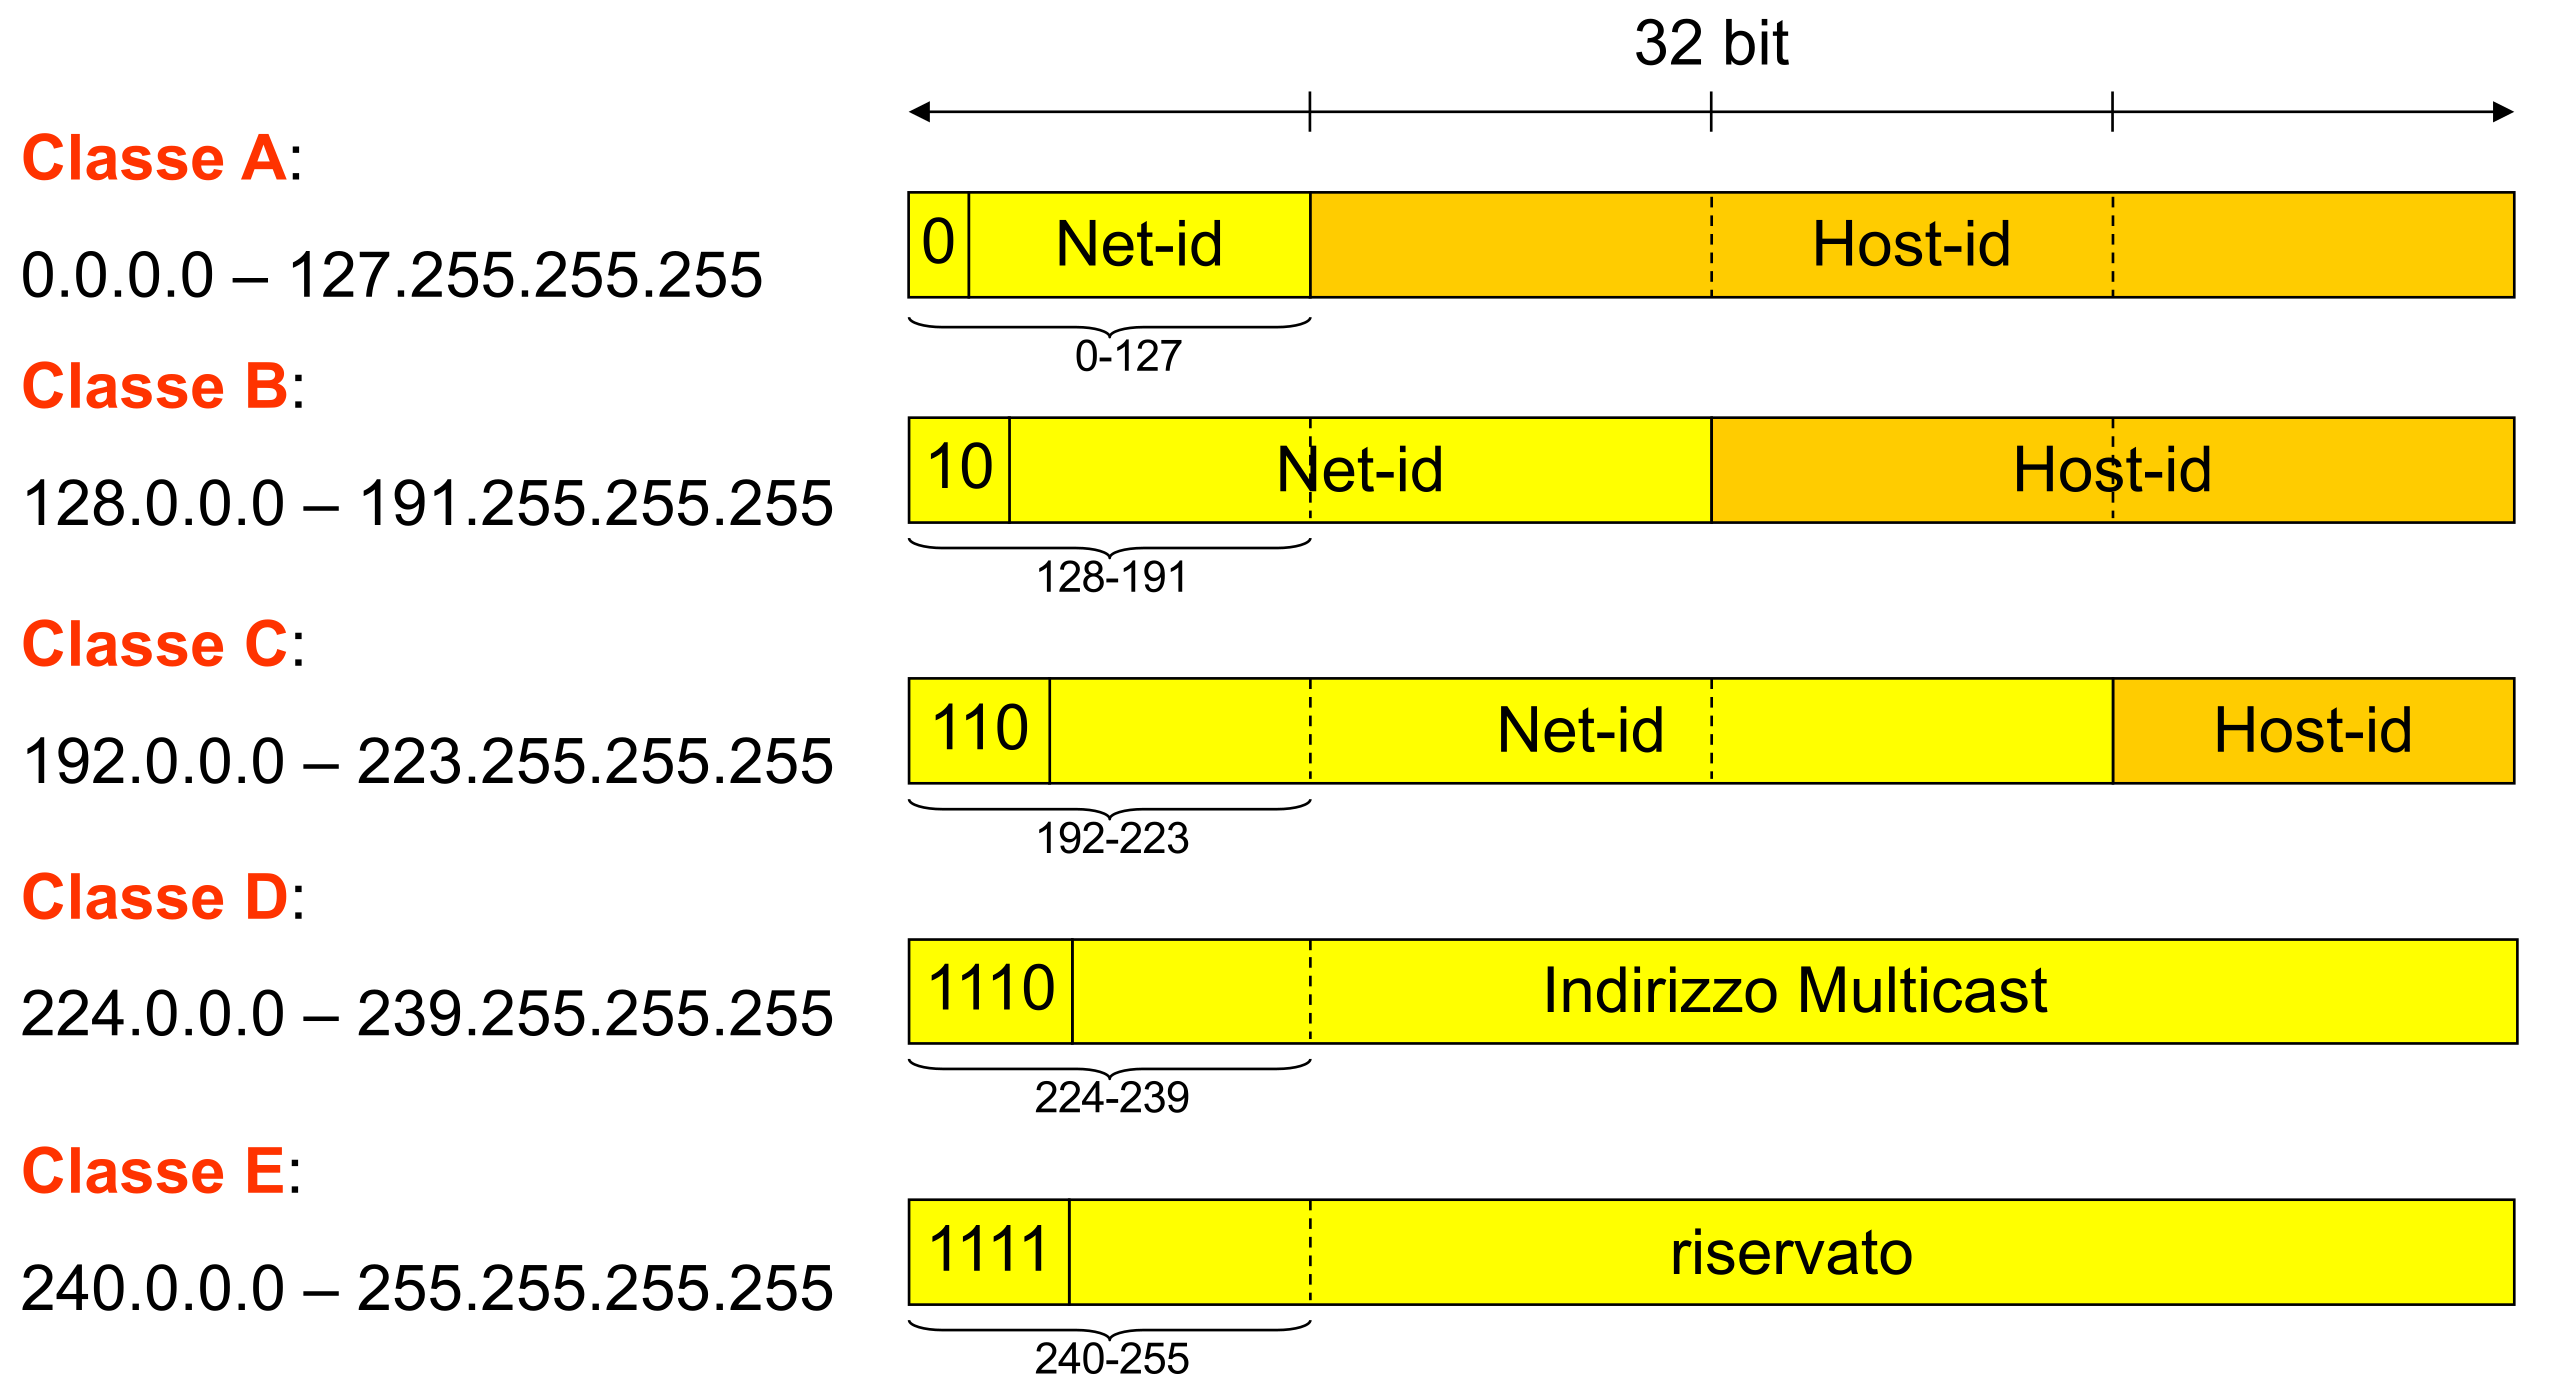
\includegraphics[width=1\textwidth]{images/classfulladdressing.png}
    \caption{Classful Addressing: suddivisione degli indirizzi IP in classi A, B, C, D, E}
    \label{fig:classfuladdressing}
\end{figure}

\subsection{Indirizzo IP - classless CIDR}

\begin{figure}[h!]
    \begin{minipage}{0.45\textwidth}
        \centering
        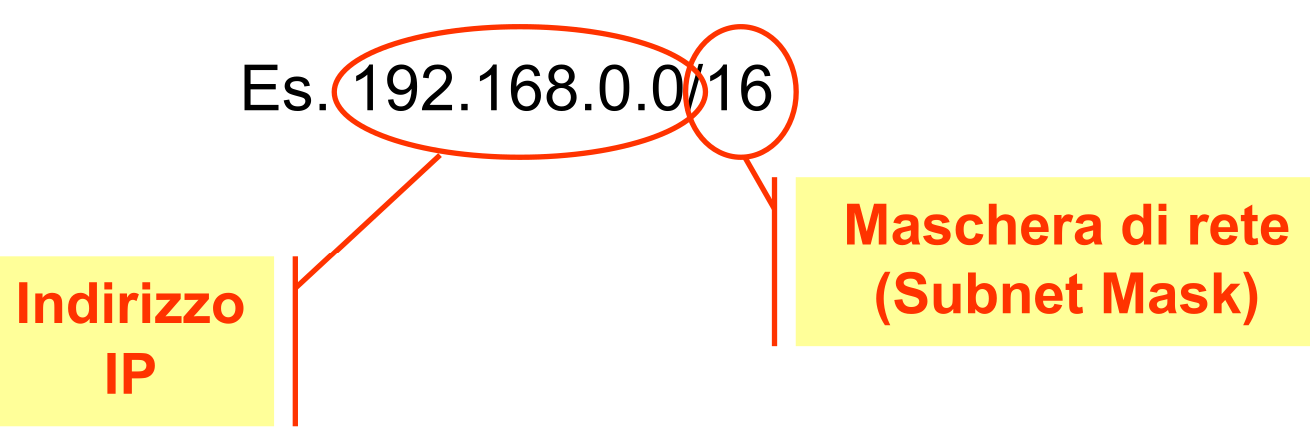
\includegraphics[width=0.95\textwidth]{images/mascheraIP.png}
        \caption{Esempio di maschera di rete (netmask) in notazione decimale e binaria}
        \label{fig:mascheraIP}
    \end{minipage}\hfill
    \begin{minipage}{0.52\textwidth}
        Il formato dell'indirizzo è del tipo \texttt{a.b.c.d/x} dove $x$ rappresenta la lunghezza della maschera di rete in bit.

        La maschera di rete permette di distinguere la parte di indirizzo relativa alla rete da quella relativa all'host. In notazione CIDR, la maschera viene indicata dopo una barra, ad esempio \texttt{192.168.1.0/24}.
    \end{minipage}
\end{figure}

\paragraph{Riconoscere un indirizzo di rete e un indirizzo di host}

Per riconoscere un indirizzo di rete e un indirizzo di host, si utilizza la maschera di rete. La maschera di rete è un numero che indica quanti bit dell'indirizzo IP sono dedicati alla parte di rete e quanti alla parte di host.

\begin{itemize}
    \item Un indirizzo di rete ha tutti zero nella parte di host.
\end{itemize}
\subsection{Subnetting}


\subsection{Classificazione degli indirizzi IP}

\subsubsection{Pubblici}
\subsubsection{Privati}

\subsubsection{Statici}
\subsubsection{Dinamici}


\subsection{Variable Length Subnet Mask (VLSM)}
\subsection{Indirizzi IP speciali}

\begin{figure}[h!]
    \centering
    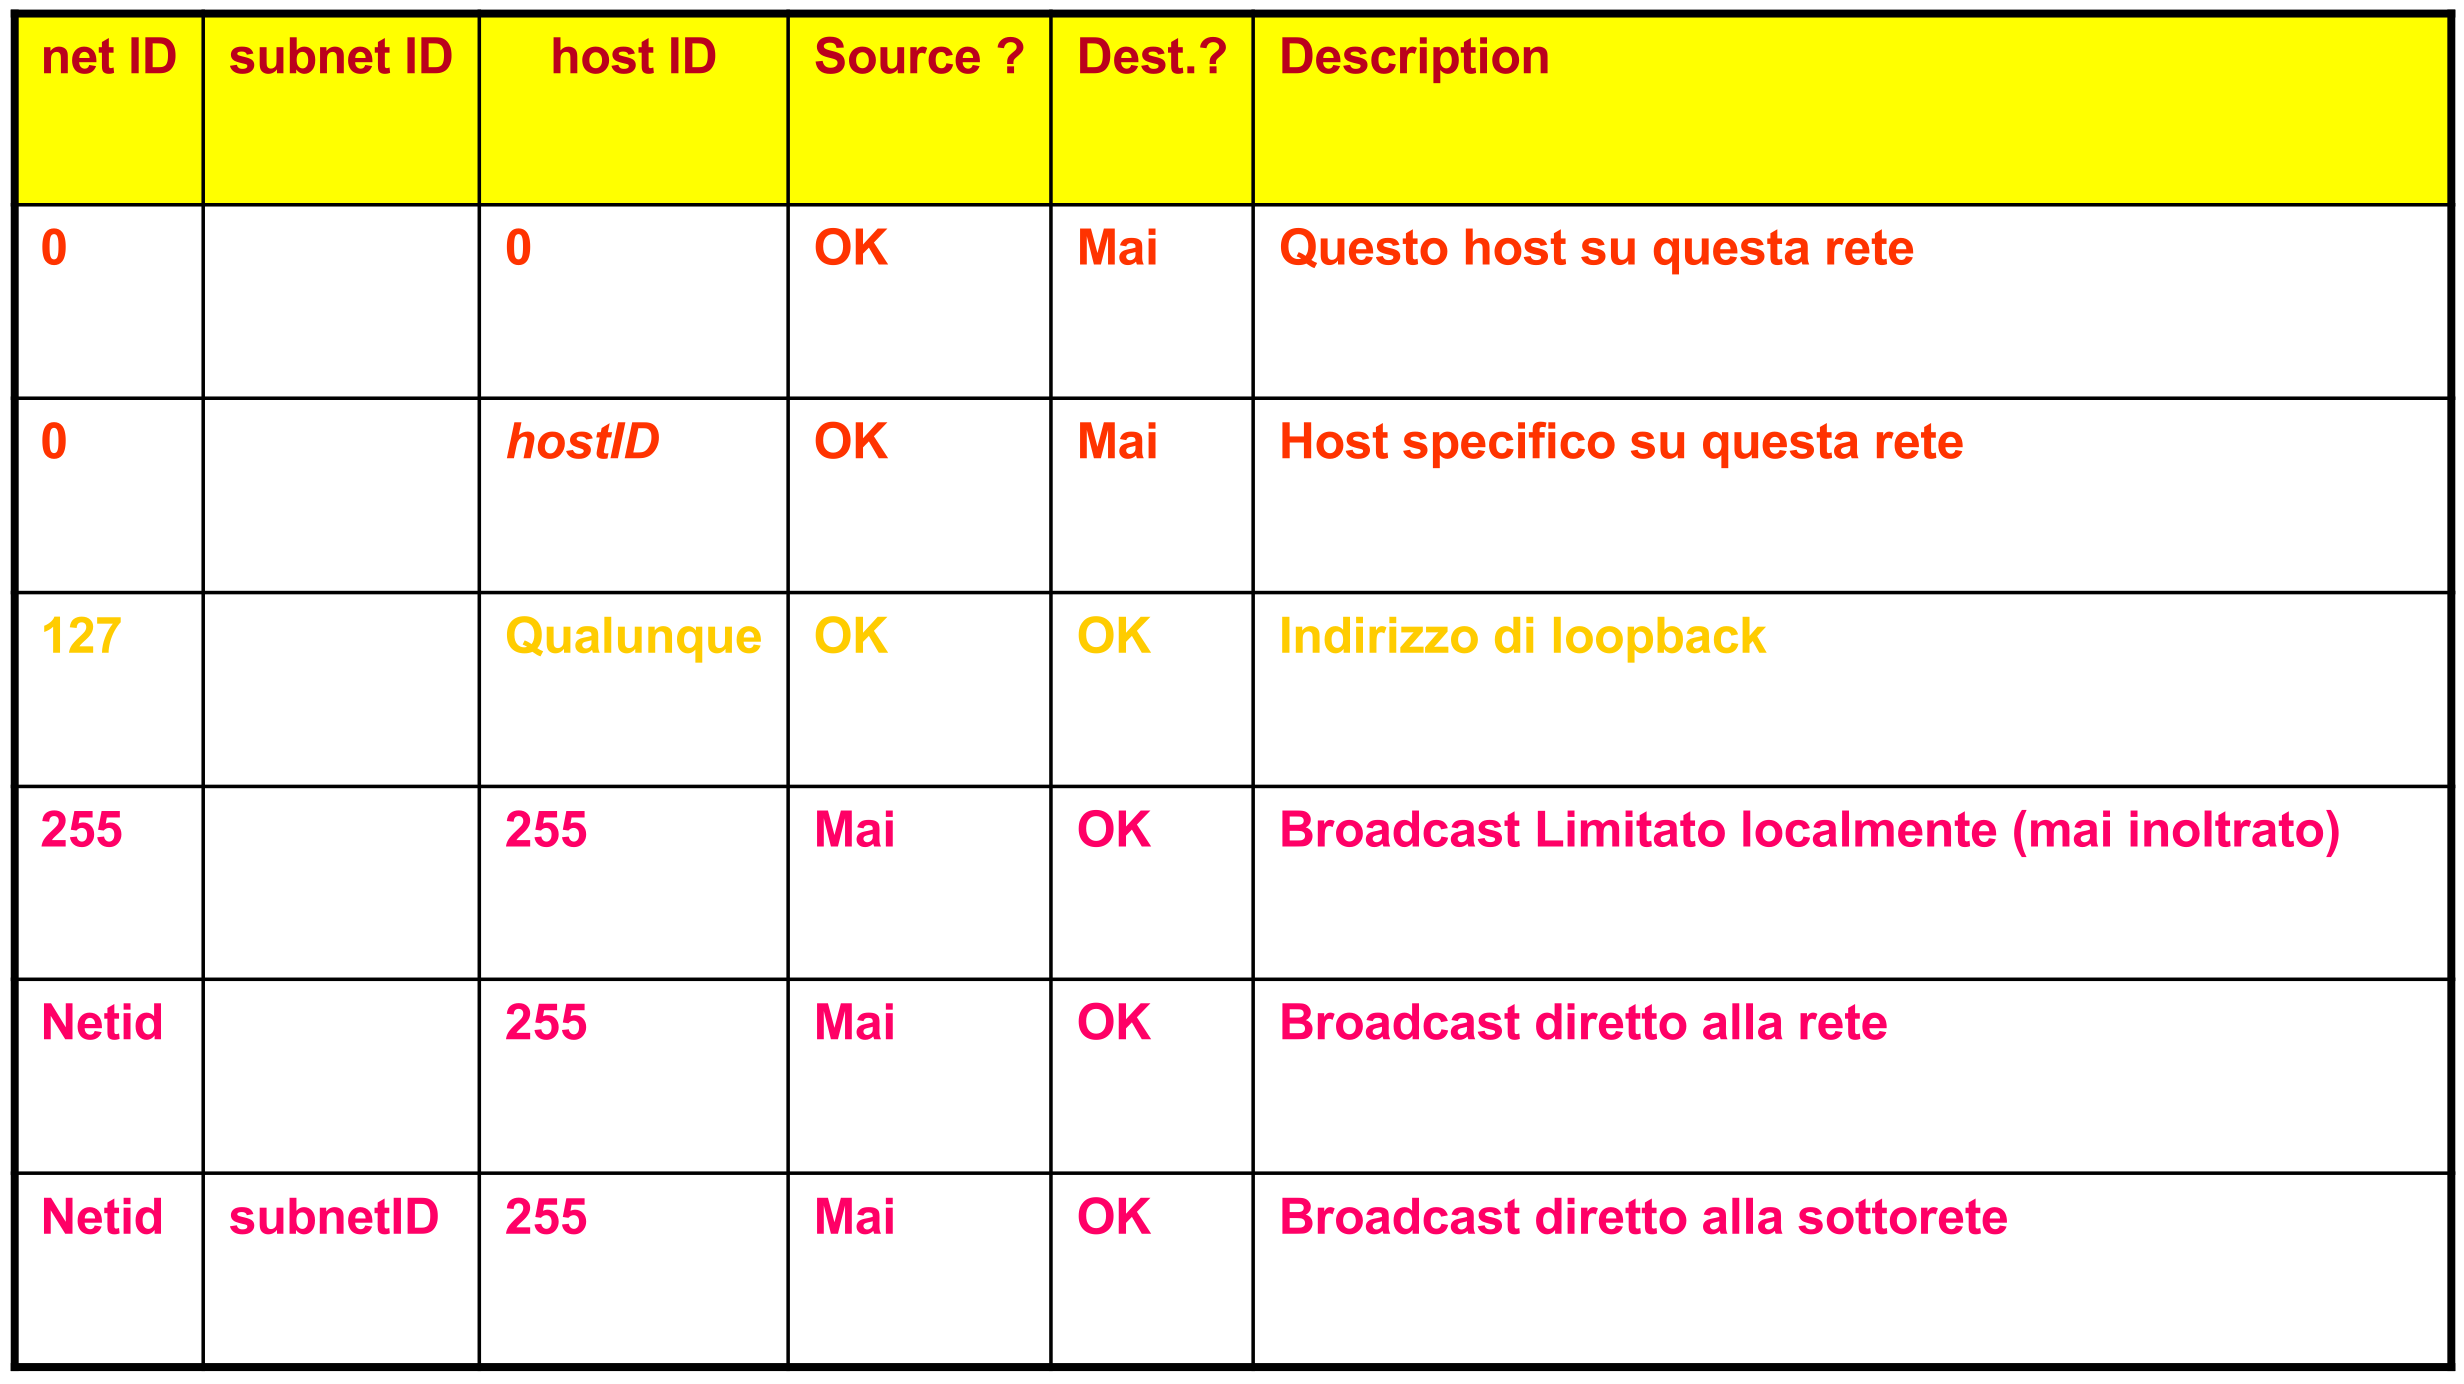
\includegraphics[width=1\textwidth]{images/indirizziipspeciali.png}
    \caption{Indirizzi IP speciali}
    \label{fig:indirizziipspeciali}
\end{figure}


\newpage
\subsection{Address Resolution Protocol (ARP) - mappatura IP a MAC}
Con ART si intende un protocollo di rete appartenente alla suite del protocollo internet (IP) versione 4 e operante a livello di accesso alla rete (livello collegamento se si considera nomenclatura ISO/OSI), il cui compito è fornire la "mappatura" tra l'indirizzo IP (32 bit - 4 byte) e l'indirizzo MAC (48 bit - 6 byte) corrispondente di un terminale in una rete locale ethernet.

Cos'è l'indirizzo MAC? 

Un indirizzo MAC (dove MAC sta per Media Access Control), detto anche "indirizzo fisico" o "indirizzo Ethernet", è un codice di 48 bit associato ad ogni dispositivo di rete che implementa lo standard Ethernet. Il suo scopo principale è quello di attribuire un'identità univoca a ciascuno dei nodi collegati ad uno stesso segmento di rete, consentendo quindi comunicazioni locali di tipo unicast. 

Al Livello 2 del modello ibrido, i pacchetti viaggiano attraverso il collegamento di più nodi, questi nodi sono caratterizzati da indirizzi fisici detti mac. 
Invece a livello tre l'indirizzo che possiede il pacchetto è !l'indirizzo definitivo!(il destinatario, non i nodi intermedi), la meta ultima del pacchetto. Però questi pacchetti viaggiano attraverso dei nodi, quindi a livello 2 i pacchetti avranno come destinazioni i nodi, e per raggiungerli hanno bisogno di conoscere gli indirizzi fisici dei nodi, perciò tramite gli indirizzi MAC e il protocollo arp si risolve il problema locale del collegamento tra i vari nodi che fanno si che il pacchetto viaggi attraverso quelli.

ARP risponde quindi a questa domanda: ho questo indirizzo ip, mi dici quale sia l'indirizzo di livello due corrispondente a questo ind ip??

Mi dice l'indirizzo del “prossimo nodo”, livello 2.

Quindi un protocollo fondamentale che individua da un indirizzo ip(liv 3) uno o più di livello 2


\begin{figure}[h!]
    \centering
    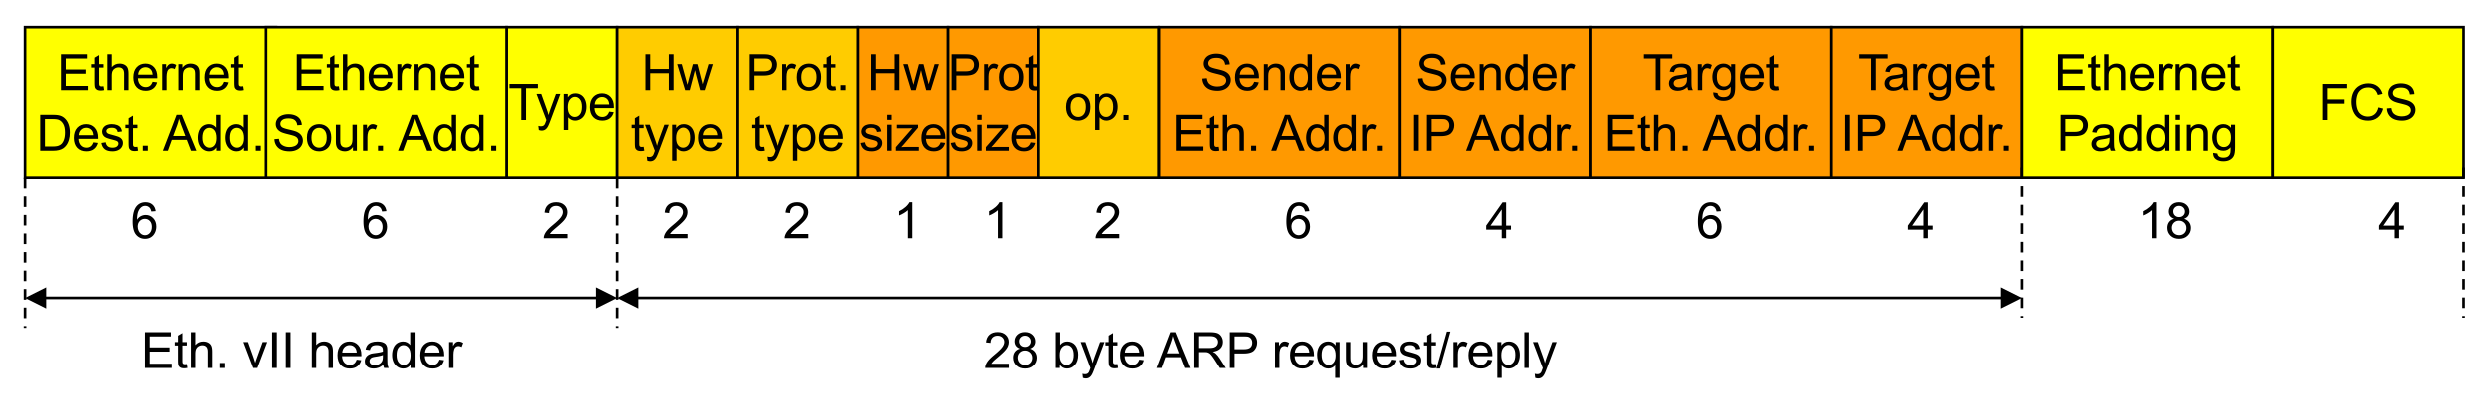
\includegraphics[width=1\textwidth]{images/frameethernet.png}
    \caption{Struttura di un frame Ethernet}
    \label{fig:frameethernet}
\end{figure}

Questo è il frame ethernet: 
in giallo ho l'header e la coda di ethernet , la coda svolge il ruolo di verificare che ci siano errori(fcs da 4 byte), il campo padding in coda serve a raggiungere i 64 byte(è un filler) minimi del frame totale tra ethernet e arp(arp è interno a l frame ethernet)
il frame deve avere una dimensione minima di 64 byte, il protocollo arp è quello arancione chiaro e scuro al centro.

Struttura del frame ethernet:
\begin{multicols}{2}
\begin{itemize}
    \item ethernet destination address: ind liv 2 del mittente - uguale a sender eth address
    \item ethernet source address
    \item type: tipologia tecnologia del livello 2
    \item hw type: specifica l'hardware che si sta usando al livello 2
    \item protocol type: specifica che procollo si vuole convertire dal liv 3 al 2(quindi non ha utilizzo esclusivo per indirizzi ip)
    \item hw size: dimensione indirizzo di liv 3
    \item prot size: dimensione indirizzo liv 2
    \item options:
    \item sender ethernet address: indirizzo liv 2 del mittente
    \item sender ip address: indirizzo liv 3 del mittente
    \item target ethernet address: indirizzo liv 2 del destinatario
    \item target ip address: indirizzo liv 3 del destinatario
    \item op: operazione che si vuole effettuare, 1 per richiesta arp, 2 per risposta arp
\end{itemize}
\end{multicols}

\subsubsection{Esempio ARP all'interno di una rete}

\begin{figure}[h!]
    \centering
    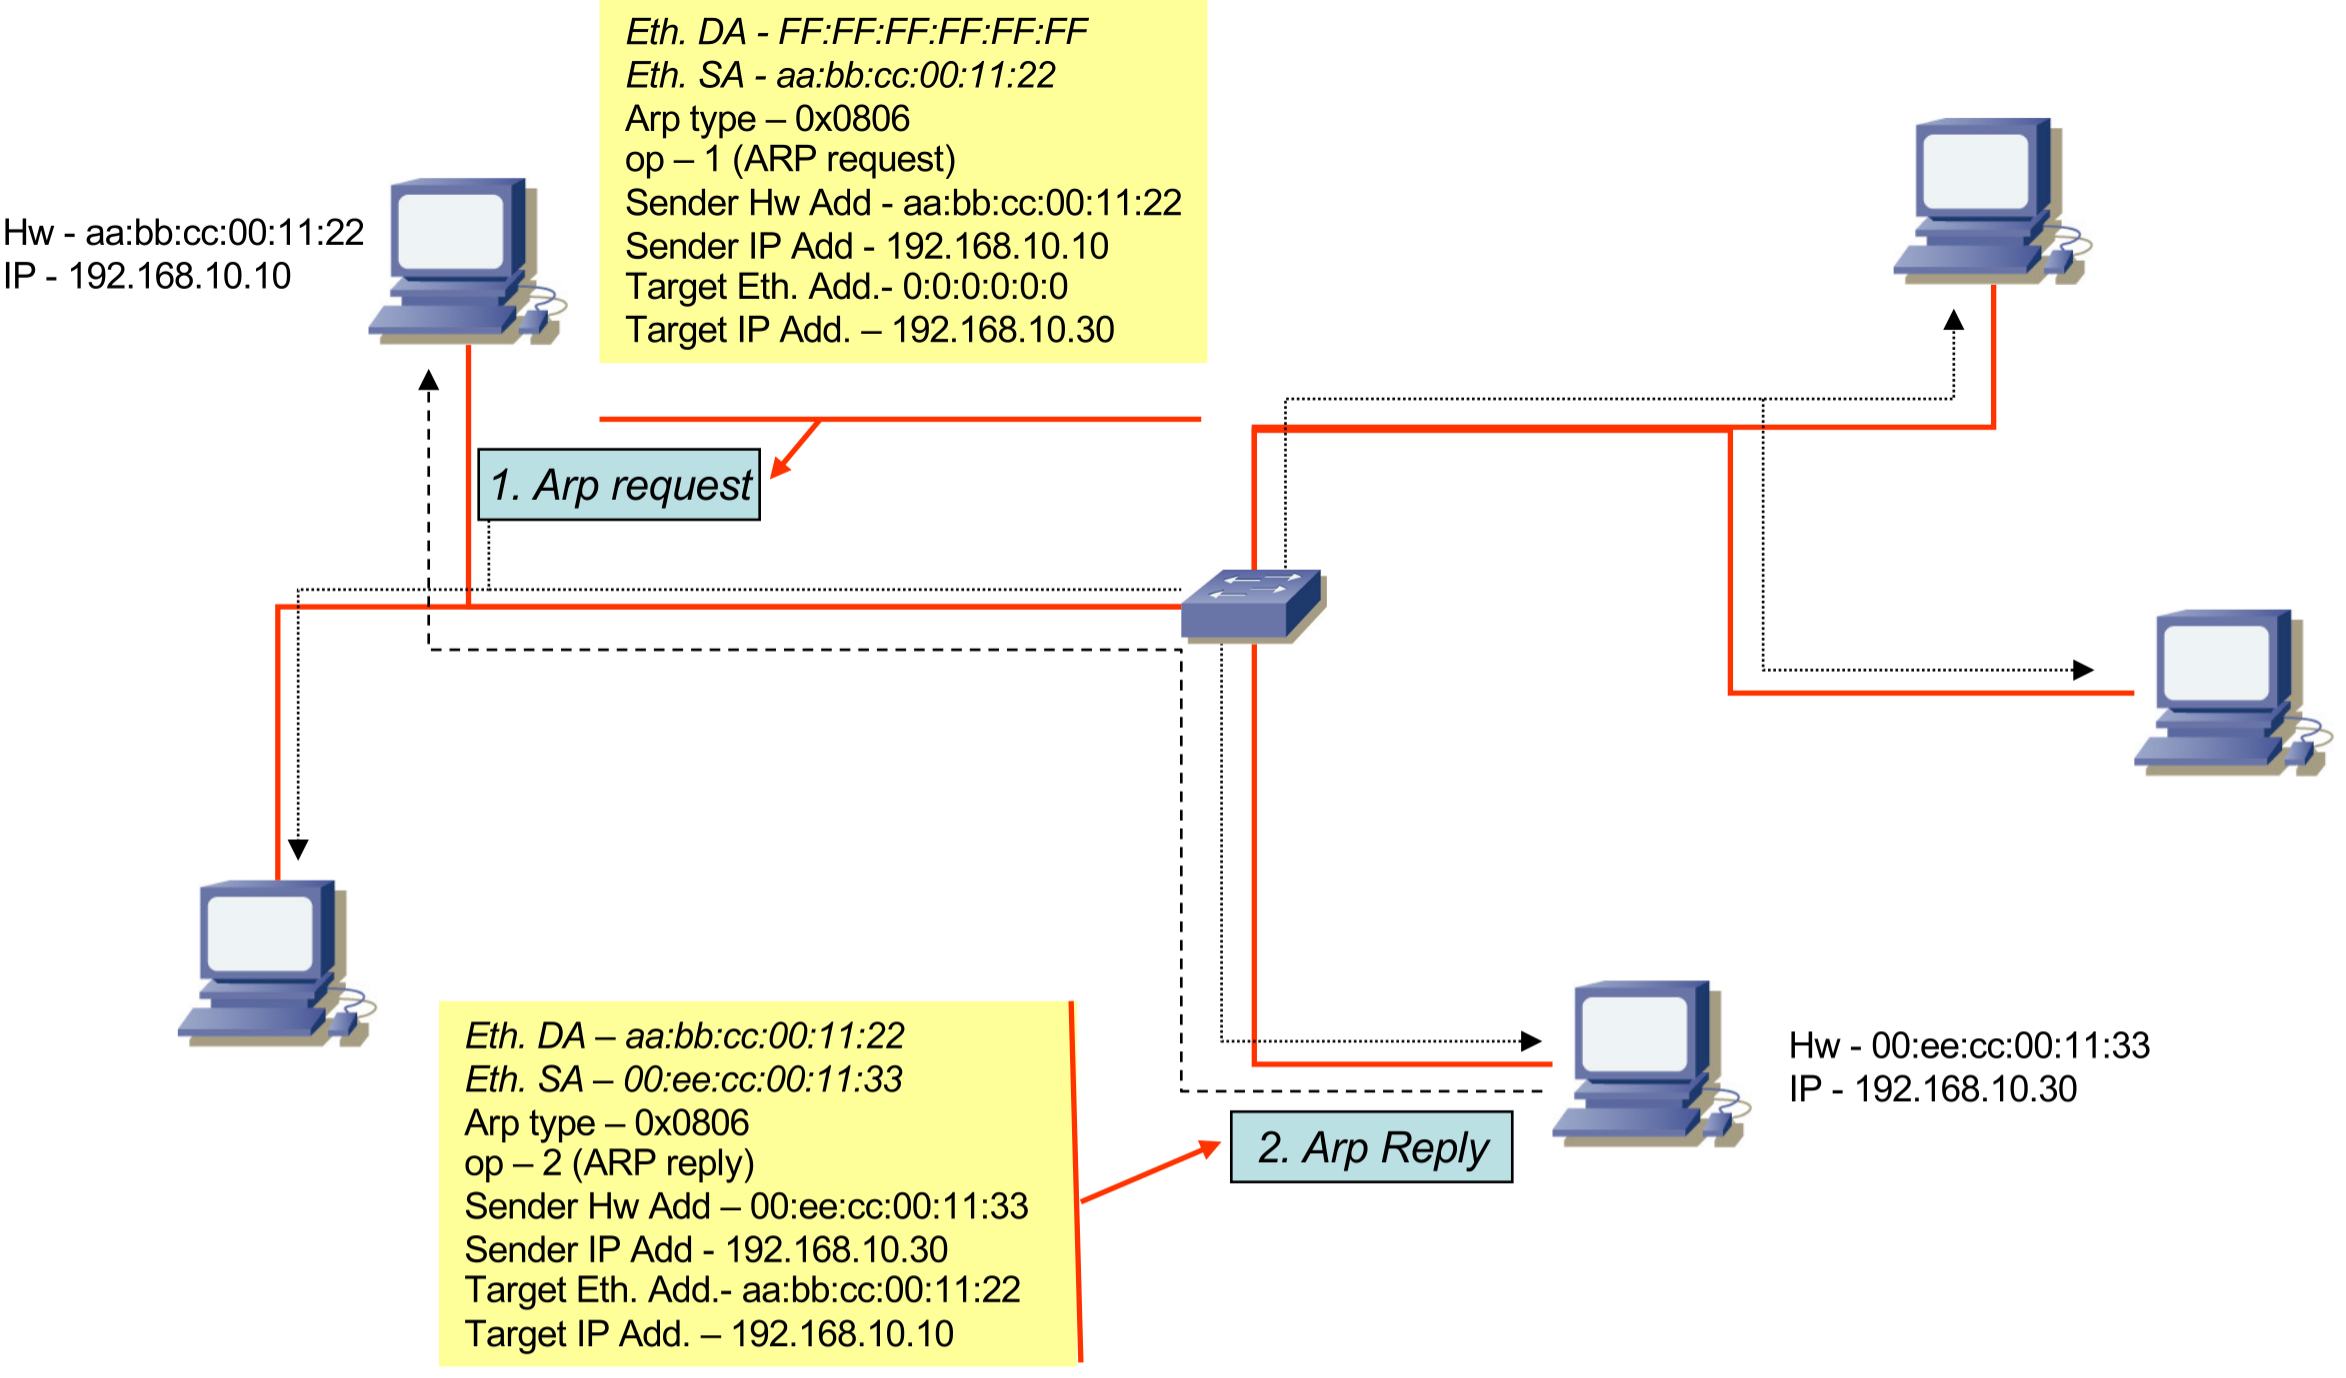
\includegraphics[width=1\textwidth]{images/esempioarp.png}
    \caption{Esempio di funzionamento del protocollo ARP}
    \label{fig:esempioARP}
\end{figure}

L'indirizzo hw è l'indirizzo fisico anche detto mac, è tipicamente in esadecimali ed è di 6 byte.

I riquadri in giallo sono pacchetti ARP utili alla comunicazione tra i due pc(visto che il dispositivo sta utilizzando arp per inviare un pacchetto allora sta usando un arp request, che viene segnato come op - 1 nel frame ethernet); i pacchetti in giallo quindi incapsulano una serie di informazioni del frame ethernet. 

Inoltre l'Ethernet destination address viene impostato a ff:ff:ff:ff:ff:ff (broadcast per indirizzi ARP) se viene effettuata un'ARP Request, questo perchè il mittente sta cercando di individuare l'indirizzo fisico del destinatario, di cui conosce solo l'ip, perciò utilzza ARP.

Nel momento della ARP request non so l'indirizzo ethernet del destinatario, ma so solo l'indirizzo ip, quindi ho tutti i byte del Ethernet address del target a 0.

Manderò quindi in broadcast(quindi multicast: a tutti i dispositivi della rete)(linee non tratteggiate) una richiesta a tutti i computer della rete, aspettando che il computer con l'indirizzo ip corrispondete a quello del target mi invii in unicast(linea tratteggiata) con un altro pacchetto ARP(arp reply, op - 2).

A questo punto il computer che ha inviato inizialmente l'ARP request riceve le info necessarie per poter inviare il pacchetto al destinatario. 
\newpage
\subsubsection{Esempio ARP in reti diverse}
IMPORTANTE: IL TCP(livello 4) si disinteressa di questo percorso, opera come se A e B fossero già collegati(end to end).

\begin{figure}[h!]
    \centering
    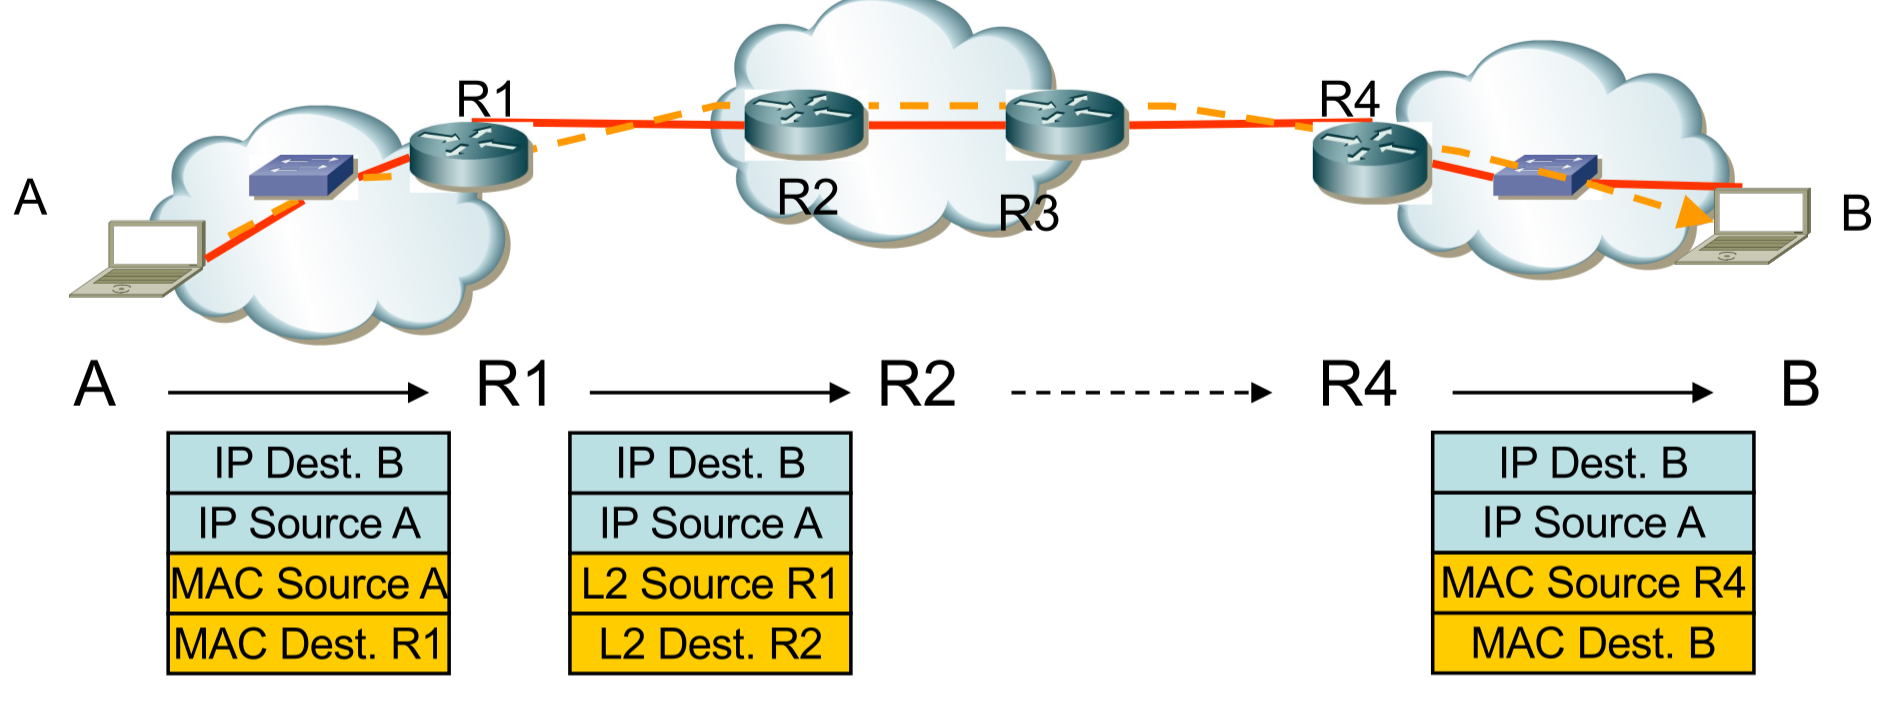
\includegraphics[width=1\textwidth]{images/esempioARPretidiverse.png}
    \caption{Esempio di funzionamento del protocollo ARP tra reti diverse}
    \label{fig:esempioARPretidiverse}
\end{figure}

\paragraph{Default gateway e tabelle di routing}

per scoprire se la rete del destinatario è la stessa da cui mando la richiesta arp: applico la mia maschera di rete all’ip del destinatario(la mia maschera di rete è un informazione che posseggo). quindi se la rete del destinatario non corrisponde a quella del mittente, per “uscire” e connettermi all’altra rete devo passare per il router. gli indirizzi di livello 3, quindi l’ip del destinatario e l’ip del mittente sono info che non variano tra un passaggio da un router all’altro, mentre quelli in giallo, gli indirizzi fisici(mac) variano tra router all’altro.
quindi il protocollo arp verrà applicato ad ogni passaggio tra un router all'altro cambiando quindi i mac source e mac destinatario, inserendo i mac dei dispositivi(router) tra cui avviene questo passaggio d’informazione. fino ad arrivare al dispositivo con l’indirizzo ip contenuto nel frame (ip dest B)
Il primo router a cui ci appoggiamo per l'inoltramento del pacchetto viene chiamato default gateway.

I router servono a connettere reti diverse, quindi se il destinatario non è nella mia rete allora mi appoggio al router, che ha un indirizzo ip di default, che è il default gateway.

Le tabelle di routing sono delle tabelle che i router utilizzano per sapere come inoltrare i pacchetti verso le reti di destinazione. Queste tabelle contengono informazioni sulle reti raggiungibili, i loro indirizzi IP e fisici.

A fine processo B legge i livelli 2 e 3 e riconosce i propri indirizzi MAC e IP, a quel punto può leggere il payload del pacchetto, che contiene i dati che A voleva inviare a B.

\paragraph{ARP nella stessa rete}
Se nel processo in cui cerco di capire se il destinatario sta nella mia rete o no scopro che sta nella mia rete allora non mi serve il router e posso inviare direttamente il pacchetto al destinatario, ma prima devo scoprire il suo indirizzo fisico(mac), quindi applico arp come fatto inizialmente.

\newpage
\subsection{Dynamic Host Configuration Protocol (DHCP) - configurazione automatica degli indirizzi IP tramite server DHCP}

 Un indirizzo ip può essere statico o dinamico, servers e router hanno tipicamente indirizzi statici.

Gli ind statici si configurano manualmente, quelli dinamici invece sono configurati tramite DHCP, un server che va configurato dall'utente ed è utile perchè fornisce: 
\begin{multicols}{3}
\begin{itemize}
    \item indirizzo ip del dispositivo
    \item netmask
    \item indirizzo ip del router
    \item indirizzo ip del server DNS
    \item lease time
\end{itemize}
\end{multicols}
Il lease time è il tempo in cui l'indirizzo ip è riservato al dispositivo, dopo di che il dispositivo deve richiedere un nuovo indirizzo ip;
è anche possibile ottenere un indirizzo IP riservato, sulla base dell'indirizzo fisico MAC.

\paragraph{DHCP relay - inoltro delle richieste DHCP}
Se nella rete locale non è disponibile un DHCP server, allora la richiesta può essere inoltrata  verso un'altra rete che dispone della funzione DHCP relay.

\paragraph{DHCP - funzionamento}
Questo protocollo fa uso dei UDP per la comunicazione tra client e server, e funziona in modo simile a ARP.

L'host che desidera un undirizzo IP si affida a questo protocollo per ottenerlo, inviando un messaggio DHCP discover, incapsulandolo in un pacchetto UDP, che viene inviato in broadcast a tutti i dispositivi della rete locale.

All'interno del pacchetto UDP, il mittente inserisce i seguenti indirizzi IP:
\begin{itemize}
    \item IP source address: l'indirizzo IP del mittente, che non è ancora stato assegnato, viene impostato momentaneamente a 0.0.0.0
    \item IP destination address: l'indirizzo IP del server DHCP, viene impostato a 255.255.255.255
\end{itemize}

Tutti gli eventuali server DHCP presenti nella rete rispondono in broadcast con un messaggio DHCP offer, che contiene le informazioni richieste dal client, come l'indirizzo IP assegnato, la netmask ecc\dots

Il client riceve le offerte dai server DHCP e sceglie una di esse, inviando un messaggio DHCP request al server scelto.

Infine il server DHCP conferma l'assegnazione dell'indirizzo IP con un messaggio DHCP ack.

    \begin{figure}[h!]
    \centering
    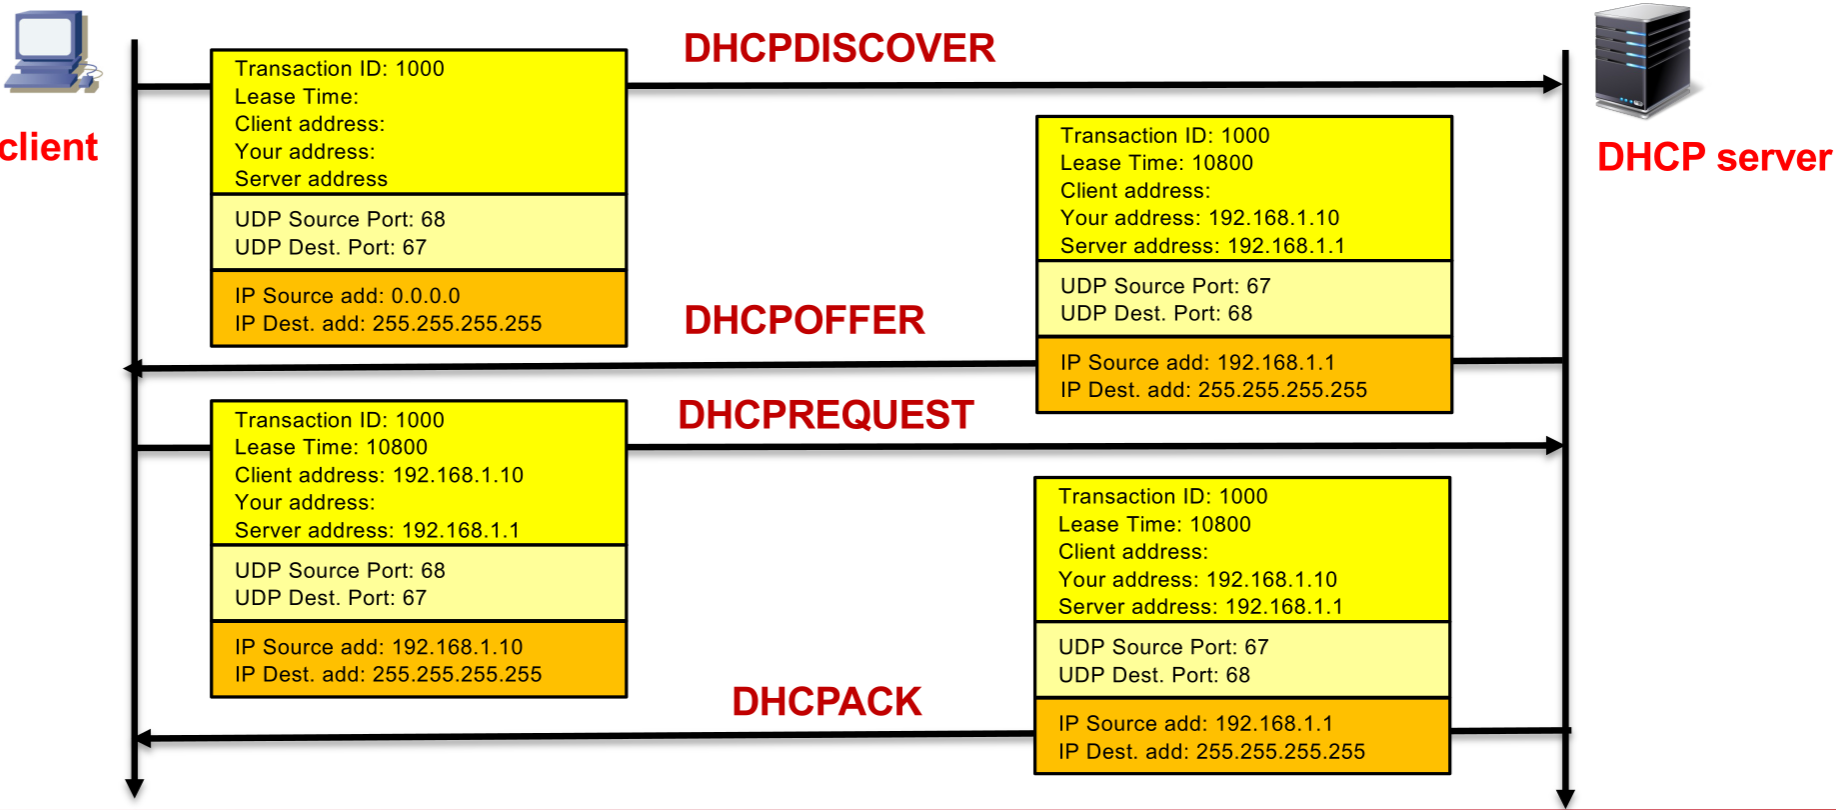
\includegraphics[width=1\textwidth]{images/dhcp.png}
    \caption{Funzionamento del protocollo DHCP}
    \label{fig:dhcp}
\end{figure}

\subsection{Zero-configuration networking}

Il zero-configuration networking è la configurazione della rete in assenza di server e amministratori, è ideale solo per reti piccole e semplici. Non è quindi un protocollo alternativo a DHCP.

\paragraph{Link-Local Address}
La IANA ha riservato a questo scopo un Link-Local Address: 169:254.0.0/16 

Gli indirizzi IP dei dispositivi nella rete vengono assegnati automaticamente, all'interno di un range specifico: [169.254.1.1 - 169.254.254]

\paragraph{ARP probe}
Quando un dispositivo si connette alla rete, invia un ARP probe per verificare se l'indirizzo IP scelto è già in uso. Se non riceve risposta, assume che l'indirizzo sia disponibile e lo utilizza. 
Se un altro host ha lo stesso indirizzo, sceglie casualmente un altro indirizzo IP all'interno dello stesso range.

\paragraph{ARP announcement}
Dopo aver scelto un indirizzo IP, il dispositivo invia un ARP announcement per informare gli altri dispositivi della rete del suo nuovo indirizzo. 

Questi indirizzi sono di tipo riservato e non possono essere usati per comunicare fuori dalla rete locale.



\subsection{Network Address Translation (NAT) - da IP privato a IP pubblico}


Il NAT è un software eseguito dal router di frontiera(ha il compito di far uscire dalla rete locale i pacchetti destinati ad indirizzi ip di altre reti).

Quindi è quel servizio che converte l'indirizzo privato del router di frontiera, in uno pubblico, cosè da comunicare con “l'esterno”. 
Perciò i router di frontiera delle altre reti non vedono l'indirizzo privato ma quello pubblico, convertito grazie al NAT.

Più precisamente, il NAT è una famiglia di tecniche/protocolli.

\paragraph{Funzionamento del NAT e tabelle di traduzione}

Tutti i datagram IP che viaggiano da (verso) la LAN hanno il medesimo indirizzo IP
mittente (destinazione), poichè il router di frontiera ha un solo indirizzo IP pubblico, che viene utilizzato per tutte le comunicazioni in uscita (entrata) dalla rete locale(LAN).

Il NAT utilizza una tabella di traduzione per mappare gli indirizzi IP privati della rete locale con l'indirizzo IP pubblico del router di frontiera; utilizzando le porte come ulteriore identificativi.

\begin{figure}[h!]
    \centering
    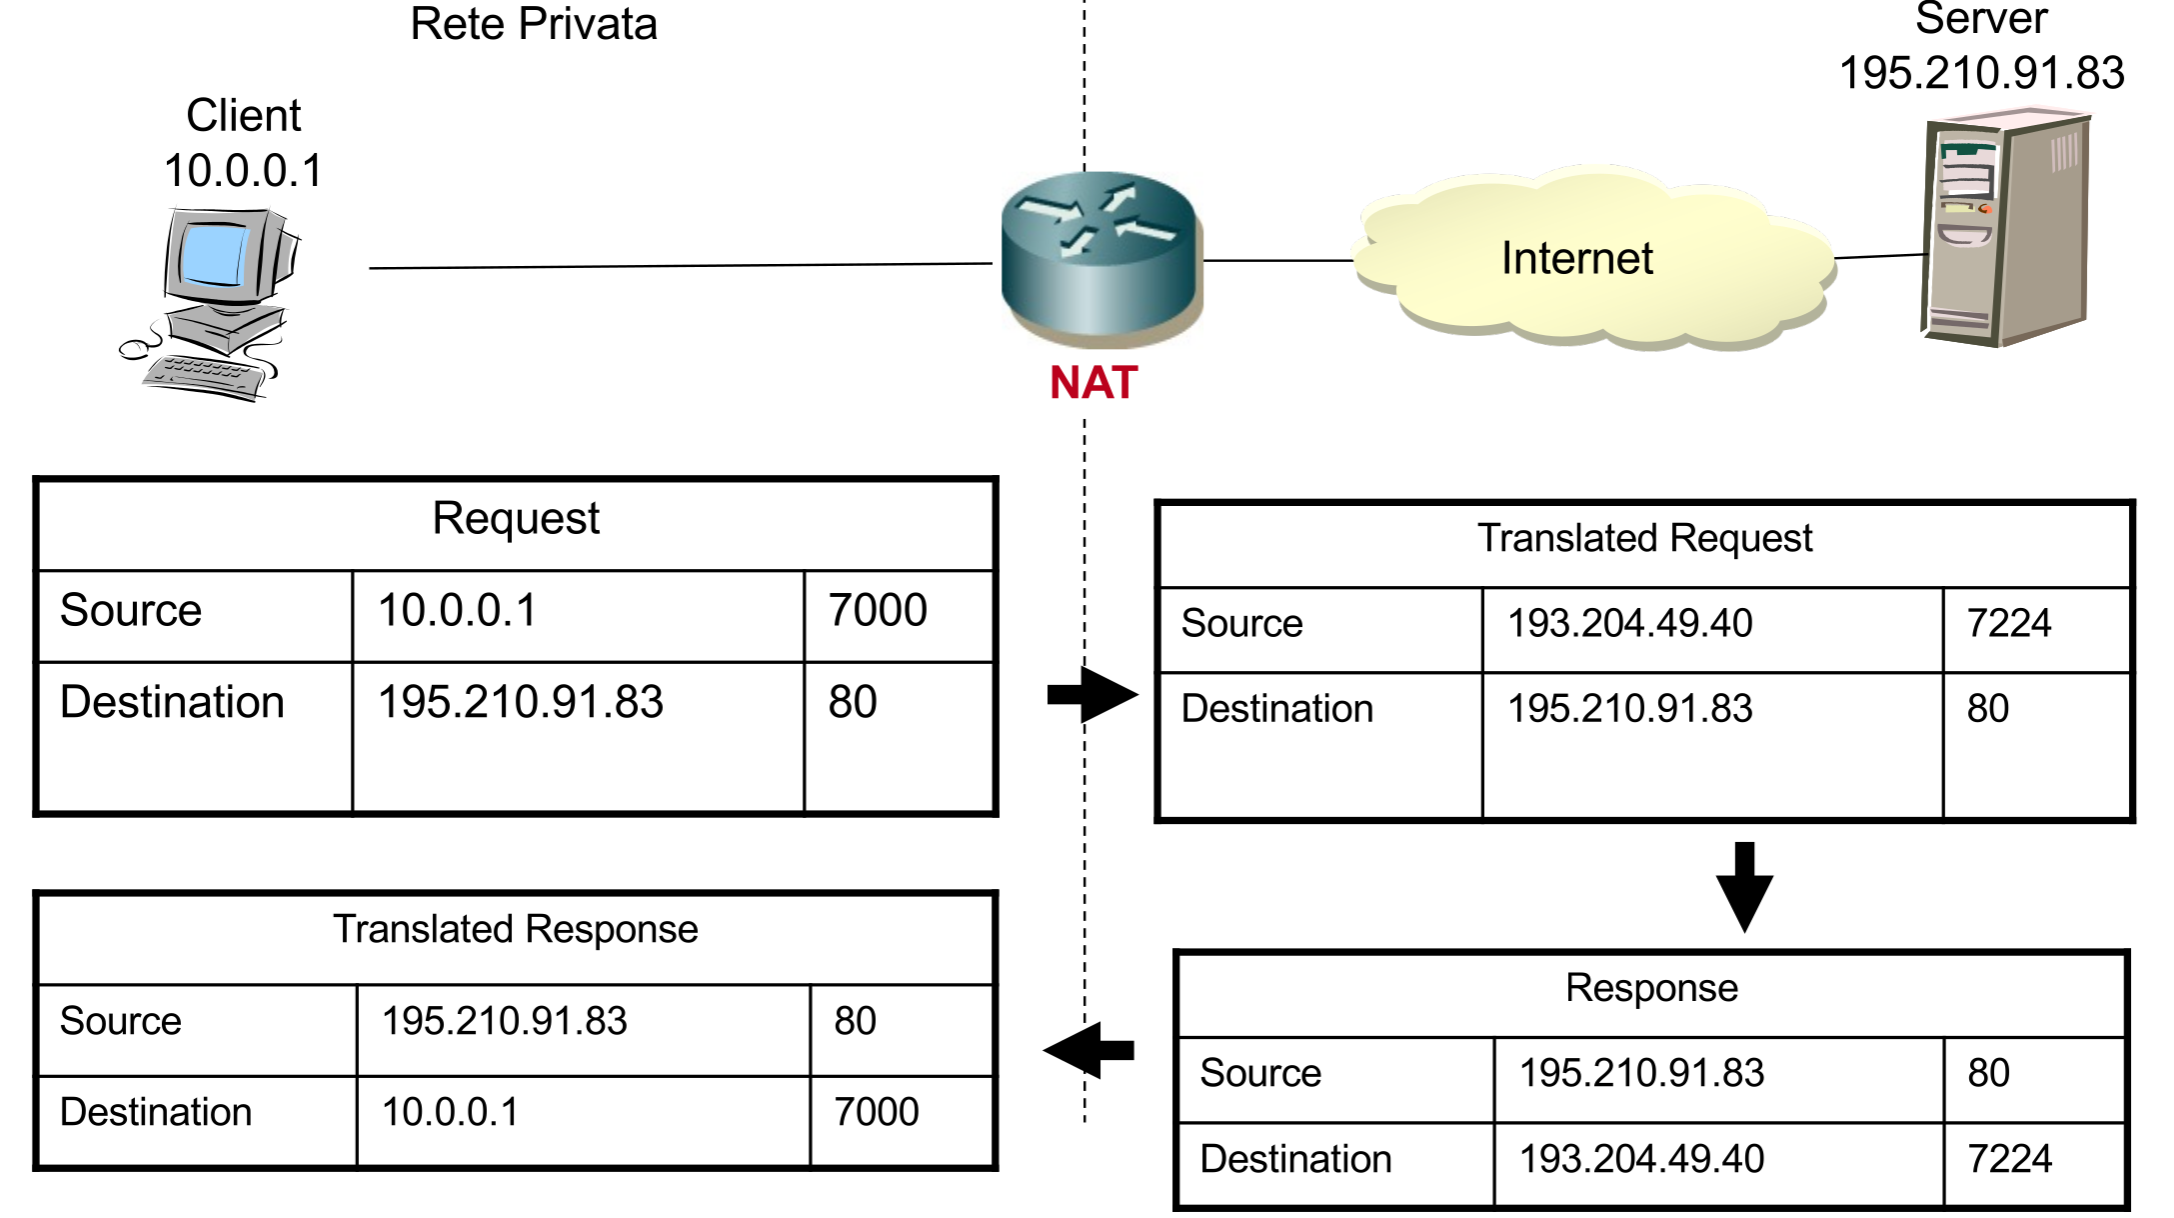
\includegraphics[width=0.85\textwidth]{images/nat.png}
    \caption{Funzionamento del NAT: traduzione degli indirizzi IP privati in indirizzi IP pubblici}
    \label{fig:nat}
\end{figure}

\newpage

\subsection{Internet control message protocol (ICMP) - diagnostica della rete}
I messaggi ICMP si dividono messaggi di errore e messaggi di richiesta; vengono inviati attraverso i pacchetti IP(protocol type 1);
questo protocollo serve a segnalare informazioni di controllo relative al livello di rete, un messaggio ICMP è composto dai campi type e code:
\begin{multicols}{2}
\begin{itemize}
    \item type: indica il tipo di messaggio ICMP
    \item code: dettagli sul tipo di messaggio
\end{itemize}
\end{multicols}


\begin{figure}[h!]
    \centering
    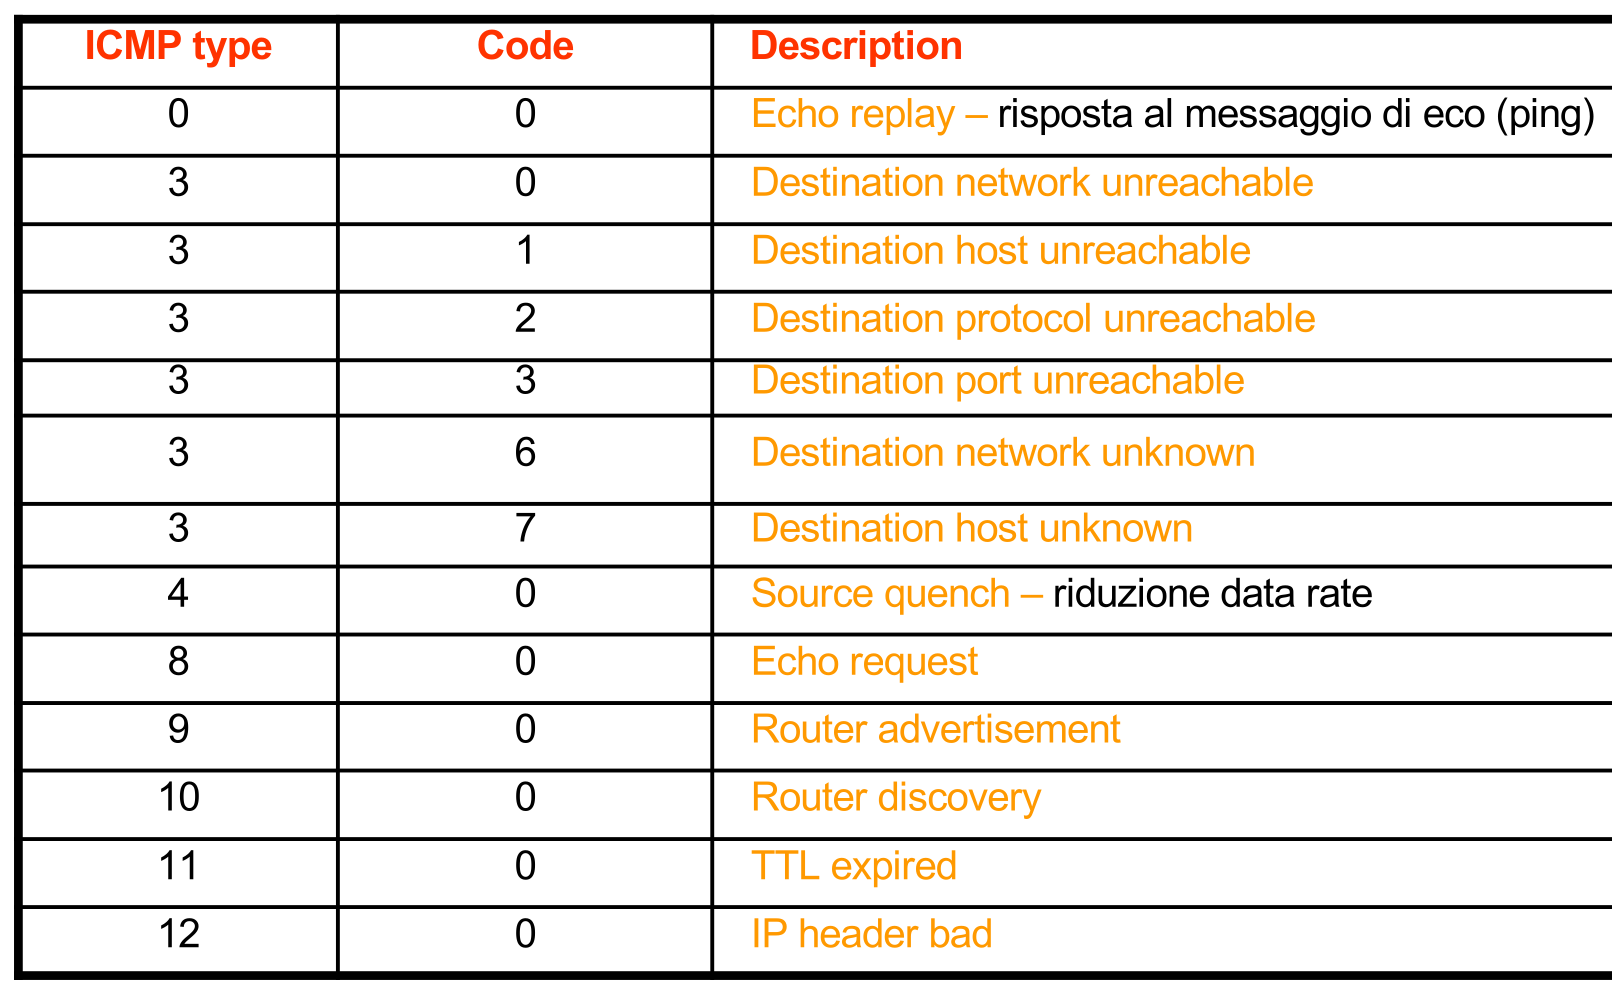
\includegraphics[width=0.67\textwidth]{images/comandiicmp.png}
    \caption{Principali comandi ICMP e loro utilizzo}
    \label{fig:comandiicmp}
\end{figure}



\paragraph{Esempio utilizzo di ICMP - ping}
Ad esempio, echo request e echo reply sono alla base del comando ping.
Type 8 corrisponde a echo request, mentre type 0 corrisponde a echo reply. 

\begin{figure}[h!]
    \centering
    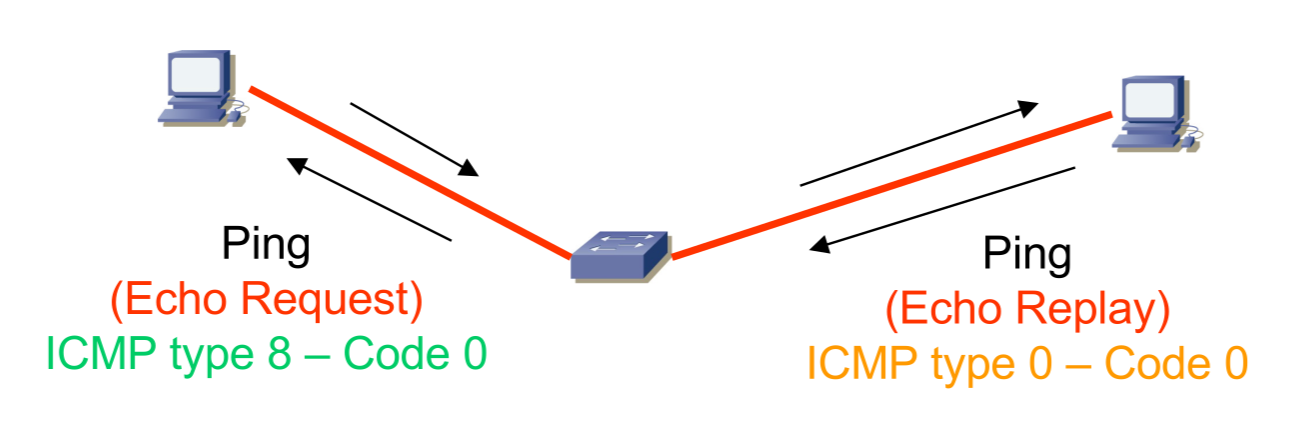
\includegraphics[width=0.55\textwidth]{images/pingicmp.png}
    \caption{Esempio di funzionamento di ICMP tramite il comando ping}
    \label{fig:pingicmp}
\end{figure}
\paragraph{Esempio utilizzo di ICMP - traceroute}
Tramite il traceroute( utilizzo dei ICMP type 11) scopro il percorso che sta seguendo il pacchetto 
comandi: traceroute sitoweb

\begin{figure}[h!]
    \centering
    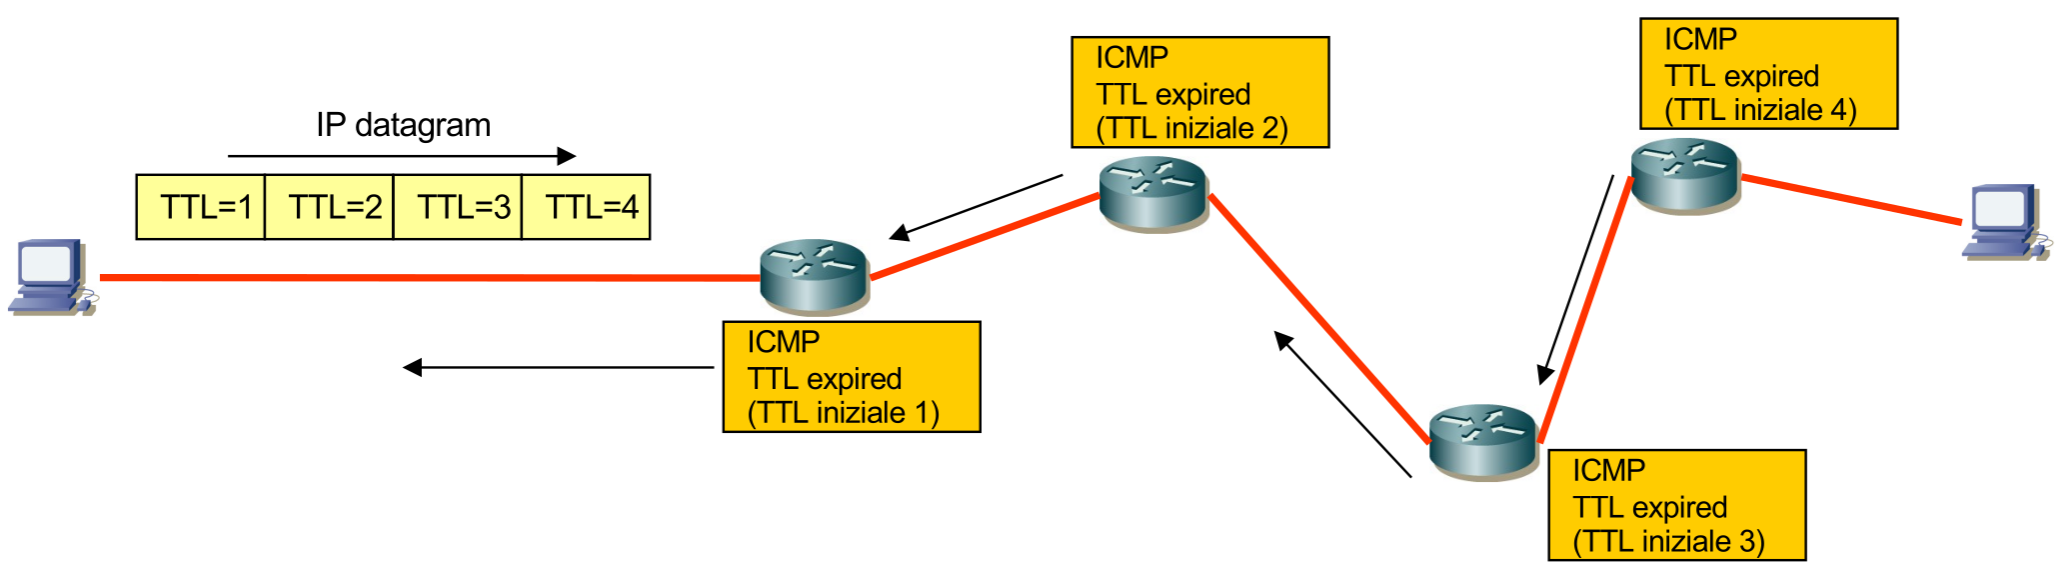
\includegraphics[width=0.8\textwidth]{images/traceroute.png}
    \caption{Esempio di funzionamento di ICMP tramite il comando traceroute}
    \label{fig:traceroute}
\end{figure}
\newpage




\section{Algoritmi di routing}


